\documentclass[12pt,a4paper]{article}

\usepackage{graphicx}

\usepackage{amsmath}
\usepackage[utf8]{inputenc}
\usepackage{listings}%pour la programmation
\usepackage{color}
\usepackage{siunitx}

\usepackage{array}

\usepackage{longtable}

\usepackage{hyperref}
\hypersetup{
    colorlinks,
    citecolor=black,
    filecolor=black,
    linkcolor=black,
    urlcolor=blue
}

\definecolor{dkgreen}{rgb}{0,0.6,0}
\definecolor{gray}{rgb}{0.5,0.5,0.5}
\definecolor{mauve}{rgb}{0.58,0,0.82}
\definecolor{red}{rgb}{0.86,0,0}
\definecolor{orange}{rgb}{1,0.47,0}

\usepackage{caption}
\DeclareCaptionLabelSeparator{colon}{ : }
\DeclareCaptionFont{white}{ \color{black} }
\DeclareCaptionFormat{listing}{
  \colorbox[cmyk]{0,0,0,0}{
    \parbox{\textwidth}{\hspace{15pt}#1#2#3}
  }
}
\captionsetup[lstlisting]{ format=listing, labelfont=white, textfont=white, singlelinecheck=false, margin=0pt, font={bf,footnotesize} }

\renewcommand{\lstlistingname}{Code source}% Listing -> Algorithm
%\renewcommand{\lstlistlistingname}{Liste des codes source}% List of Listings -> List of Algorithms

\usepackage{inconsolata}%pour changer la police typewriter (machine à écrire)

\lstnewenvironment{java}{
\lstset{frame=tb,
  language=Java,
  aboveskip=3mm,
  belowskip=3mm,
  showstringspaces=false,
  columns=flexible,
  basicstyle={\small\ttfamily},
  numbers=none,
  numberstyle=\tiny\color{gray},
  keywordstyle=\color{blue},
  commentstyle=\color{dkgreen},
  stringstyle=\color{mauve},
  breaklines=true,
  breakatwhitespace=true,
  tabsize=3,
  mathescape=true
}
}{}
\usepackage{etoolbox}

\lstnewenvironment{arduino}{
%% http://tex.stackexchange.com/questions/32174/listings-package-how-can-i-format-all-numbers
\lstdefinestyle{Arduino}{%
    aboveskip=3mm,
    belowskip=3mm,
    showstringspaces=false,
    columns=flexible,
    basicstyle={\small\ttfamily},
    language=C,
    emph={String, Servo, delay, substring, write, toInt, digitalWrite, Serial, readString, println, sizeof, pinMode, attach},%                 define keywords
    morecomment=[l]{//},%             treat // as comments
    morecomment=[s]{/*}{*/},%         define /* ... */ comments
    keywords={HIGH, OUTPUT, LOW, void, int, for, if, else, while},%        keywords to emphasize
    numberstyle=\tiny\color{gray},
	keywordstyle=\color{blue},
	commentstyle=\color{red},
	stringstyle=\color{mauve},
	emphstyle=\color{orange},
	breaklines=true,
  	breakatwhitespace=true,
  	tabsize=3
}
\lstset{
	style=Arduino,
	mathescape=true
}
}{}

\lstnewenvironment{python}{
	\lstset{frame=tb,
	  language=Python,
	  aboveskip=3mm,
	  belowskip=3mm,
	  showstringspaces=false,
	  columns=flexible,
	  basicstyle={\small\ttfamily},%\small ??
	  numbers=none,
	  numberstyle=\tiny\color{gray},
	  keywordstyle=\color{orange},
	  commentstyle=\color{red},
	  stringstyle=\color{mauve},
	  breaklines=true,
	  breakatwhitespace=true,
	  tabsize=3,
	  mathescape=true
	}
}{}
%utf-8
\lstset{literate=
  {á}{{\'a}}1 {é}{{\'e}}1 {í}{{\'i}}1 {ó}{{\'o}}1 {ú}{{\'u}}1
  {Á}{{\'A}}1 {É}{{\'E}}1 {Í}{{\'I}}1 {Ó}{{\'O}}1 {Ú}{{\'U}}1
  {à}{{\`a}}1 {è}{{\`e}}1 {ì}{{\`i}}1 {ò}{{\`o}}1 {ù}{{\`u}}1
  {À}{{\`A}}1 {È}{{\'E}}1 {Ì}{{\`I}}1 {Ò}{{\`O}}1 {Ù}{{\`U}}1
  {ä}{{\"a}}1 {ë}{{\"e}}1 {ï}{{\"i}}1 {ö}{{\"o}}1 {ü}{{\"u}}1
  {Ä}{{\"A}}1 {Ë}{{\"E}}1 {Ï}{{\"I}}1 {Ö}{{\"O}}1 {Ü}{{\"U}}1
  {â}{{\^a}}1 {ê}{{\^e}}1 {î}{{\^i}}1 {ô}{{\^o}}1 {û}{{\^u}}1
  {Â}{{\^A}}1 {Ê}{{\^E}}1 {Î}{{\^I}}1 {Ô}{{\^O}}1 {Û}{{\^U}}1
  {œ}{{\oe}}1 {Œ}{{\OE}}1 {æ}{{\ae}}1 {Æ}{{\AE}}1 {ß}{{\ss}}1
  {ç}{{\c c}}1 {Ç}{{\c C}}1 {ø}{{\o}}1 {å}{{\r a}}1 {Å}{{\r A}}1
  {€}{{\EUR}}1 {£}{{\pounds}}1
}

\author{Quentin Barri\`ere, Gr\'egoire Charleux, Yannis Lamoussi\`ere,\\ Mathis Pastorelli \\[0.2cm]
\emph{Lycée Pierre de Fermat}}
\date{\(2016-2017\)}

\renewcommand{\contentsname}{Sommaire}

\renewcommand{\figurename}{Illustration}
\renewcommand{\tablename}{Tableau}

\renewcommand{\listfigurename}{Liste des illustrations}
\renewcommand{\listtablename}{Liste des tableaux}

\setcounter{secnumdepth}{5}
\setcounter{tocdepth}{5}

\begin{document}
	\title{\Huge Dossier de pr\'esentation de TPE \\ ------------ \\ \Large Robot d'assistance \`a localisation par reconnaissance faciale}
	\maketitle
	
	\newpage
	
	\tableofcontents
	
	\newpage
	
	\section{Présentation du projet}
	
	\subsection{L'idée}
	
	Notre TPE a pour thème la robotique, ce qui signifie que l'un des buts de ce projet était d'aboutir à la construction d'un robot. En effet les systèmes robotisés sont de plus en plus utilisés de nos jours et ils couvrent à peu près tous les domaines de la vie courante. Nous avons choisi la problématique suivante : comment aider nos grands-parents à limiter leur trajet et effort en transportant, automatiquement, leurs objets les plus usuels à l’intérieur de leur maison ?
	
	\subsection{Historique}
	
\indent\indent L’idée fut trouvée par Mathis Pastorelli après que notre professeur de SI nous a déconseillé de choisir le projet précédent.
En effet en premier lieu nous avions choisi comme problématique : est-il possible qu’un avion solaire soit entièrement autonome ? Cette idée nous était venu grâce à Solar Impulse et d’autres nouvelles technologies comme lui. Seulement, notre professeur nous à clairement fait comprendre que nous n’arriverions à rien faire et que notre projet été impossible. Nous avons donc cherché un  autre sujet, et Mathis Pastorelli nous a proposé celui-ci. 
Dans un premier temps notre robot devait fonctionner avec des ultrasons. L’utilisateur devait posséder une télécommande assurant la communication avec le robot. Tout d’abord, l’utilisateur devait envoyer un ultrason au robot afin de le communiquer son envie d’être localisé. Après la réception du signal, le robot renvoie un ultrason à la télécommande qui lui en renvoie une autre dès sa réception. Cet échange permet au robot de calculer la distance le séparant de son utilisateur. Après cet échange, le robot devait se déplacer d’une distance près définie et donc connue, et effectuer un nouvel échange avec la télécommande afin d’obtenir une nouvelle information sur la distance le séparant de son utilisateur. Après avoir effectué toutes ces mesures, le robot connaît donc les trois distances, lui permettant de faire un triangle et donc de déterminer ses angles grâce à une des applications du théorème d’Al-Kashi. Celui-ci dit que dans un triangle $ABC$ ayant $\alpha$, $\beta$ et $\gamma$ pour angles et $a$, $b$ et $c$ pour longueurs de côtés respectivement opposés à ces angles on a : $c^2 = a^2 + b^2 – 2ab.cos(\gamma)$. L'application que nous avons trouvée de ce théorème permet de calculer un de ses angles. Si on considère $c$ comme la première distance déterminée par l’échange d’ultrasons, $a$ la distance de déplacement du robot prédéfinie et $b$  la seconde distance déterminée par échange d’ultrasons, il nous fallait donc déterminer l’angle $\gamma$ qui aurait été l’angle de rotation des roues. Et pour cela nous voulions utiliser cette formule déduite du théorème lui-même : $$\gamma = arccos\left(\dfrac{a^2 + b^2 - c^2}{2ab}\right) $$
	\newpage
	\section{Système souhaité}
	
	Après avoir réalisé le cahier des charges et défini nos principaux objectifs ainsi que les tâches que devra accomplir notre robot nous avons trouvé plusieurs solutions techniques pour le rendre efficace.
Nous avons réalisé une série de schémas qui nous ont permis de synthétiser ces solutions techniques :

	\subsection{Diagramme des interacteurs (diagramme pieuvre)}

Nous avons défini les différentes fonctions contraintes, liées aux éléments extérieurs, qui affecteront le robot :

	\begin{figure}[ht!]
		\centering
			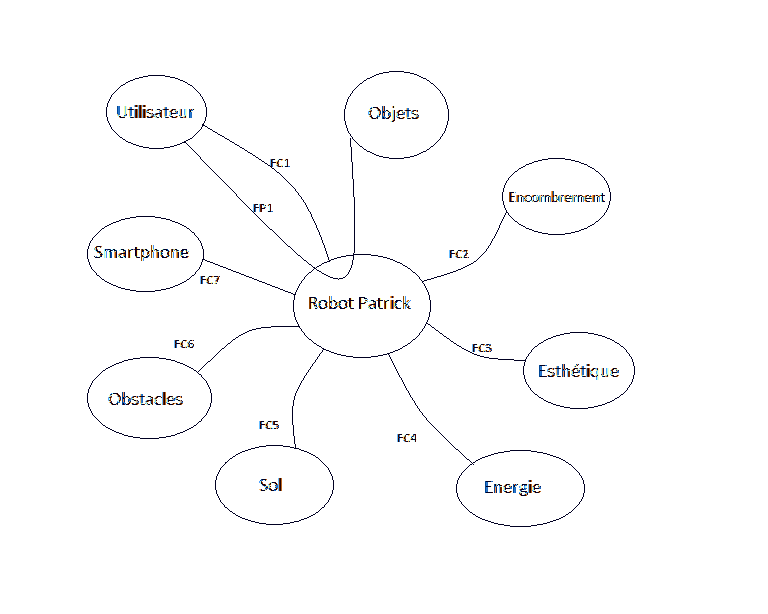
\includegraphics[width=90mm]{Diagramme_pieuvre.png}
			\caption[Diagramme des interacteurs - Illustration réalisée par notre groupe, disponible à l'adresse : \url{https://github.com/thaspdev/PATRICK/illustrations/Diagramme_pieuvre.png}]{Diagramme des interacteurs\label{overflow}}
	\end{figure}

Ce diagramme nous a permis d'identifier la fonction principale et les fonctions contraintes du robot :\\
\indent - FP1: apporter des objets à l'utilisateur\\
\indent - FC1 : apporter un certain volume et une certaine quantité d'objets\\
\indent - FC2 : ne pas être trop encombrant\\
\indent - FC3 : plaire à l'utilisateur\\
\indent - FC4 : avoir une bonne autonomie\\
\indent - FC5 : s'adapter au sol\\
\indent - FC6 : éviter les obstacles\\
\indent - FC7 : être contrôlable avec un smartphone\\


	\subsection{Diagramme FAST (analyse des fonctions du système)}

\indent \indent Nous avons représenté les solutions techniques appropriées à chacune des fonctions de service permettant de réaliser la fonction principale (apporter des objets à l'utilisateur) :

\begin{center}
\renewcommand{\arraystretch}{1.2}
\begin{longtable}{|>{\small}m{3cm}|>{\small}c|}
\hline
FP1 : Apporter des objets à l’utilisateur & \begin{tabular}{@{}m{3cm}|c@{}}
FT1 : Alimenter le système en énergie &ST1 : accumulateur + 2 piles 9V\\
\hline
FT2 : Repérer l’utilisateur & \begin{tabular}{@{}m{3cm}|m{3cm}@{}}
FT21 : Voir l'utilisateur & ST21 : Caméra\\
\hline
FT22 : Orienter la caméra & ST22 : Moteur pas à pas+servo moteur
\end{tabular}\\
\hline
FT3 : Gérer les informations & \begin{tabular}{@{}m{3cm}|m{3cm}@{}}FT31 : Traiter les informations provenant de la caméra &ST3 : cartes électroniques (raspberry pi)
\end{tabular}\\
\hline
FT4 : Se déplacer jusqu’à l’utilisateur & \begin{tabular}{@{}m{3cm}|m{3cm}@{}}
FT41 : Orienter les roues &ST41 : 2 servomoteurs\\
\hline
FT42 : Transformer l’énergie électrique en énergie mécanique de rotation &ST42 : Moteur électrique\\
\hline
FT43 : Adapter la vitesse &ST43 : Réducteur à engrenages\\
\hline
FT44 : Être en contact avec le sol &ST44 : 2 roues motrices+4 roues stabilisatrices\\
\end{tabular}\\
\hline
(FT5 : Éviter les obstacles) & \begin{tabular}{@{}m{3cm}|m{3cm}@{}}
FT51 : Détecter les obstacles&ST51 : 4 émetteurs / récepteurs d’ultrasons\\
\hline
FT52 : Gérer les informations&ST52 : cartes électroniques (mêmes que ST3)\\
\hline
FT53 : Modifier la trajectoire&ST53 : servomoteurs (mêmes que ST42)\\
\end{tabular}\\
\hline

\end{tabular}\\
\hline
FP1 : Apporter des objets à l’utilisateur & \begin{tabular}{@{}m{3cm}|c@{}}
FT6 : S’arrêter près de l’utilisateur& \begin{tabular}{@{}m{3cm}|m{3cm}@{}}
FT61 : Déterminer la distance à parcourir&\begin{tabular}{@{}m{3cm}@{}}
ST61 : caméra\\
\hline
ST61 bis : bouton poussoir\\
\end{tabular}\\
\hline
FT62 : Arrêter le mouvement &ST62 : moteur + roues\\
\end{tabular}\\
\end{tabular}\\
\hline
\caption{Diagramme FAST\label{overflow}}
\end{longtable}
\end{center}

Ainsi nous avons pu établir la liste des principaux composants de notre futur robot :

- un accumulateur pour stocker son énergie ;

- une caméra qui pivote grâce à un moteur pas à pas et à un servomoteur afin de repérer l'utilisateur ;

- 2 cartes électroniques (Raspberry Pi + Arduino), qui communiquent entre elles pour gérer les informations et commander tous les composants ;

- 2 servomoteurs pour orienter l'ensemble roues motrices/ moto réducteur (un horizontal et un vertical) ;

- un moteur électrique servant à faire avancer le robot en faisant tourner les 2 roues motrices par le biais d'un réducteur à engrenages permettant d'augmenter son couple en réduisant sa vitesse de rotation ;

- 4 roues folles situées aux 4 coins de la base du robot pour le maintenir en équilibre et supporter sa masse ;

- 4 émetteurs/récepteurs d'ultrasons permettant de repérer les obstacles par réflexion de leurs ondes afin de les contourner;

- 4 boutons poussoirs permettant à l'utilisateur de contrôler le robot directement et un écran LCD afin de visualiser le menu du robot.


\subsection{Diagramme fonctionnel}

\indent \indent Nous avons schématisé le fonctionnement du système en représentant les différentes interactions entre les composants de la chaîne d'information (commande) et de la chaîne d'énergie (puissance) :
	\begin{figure}[ht!]
		\centering
			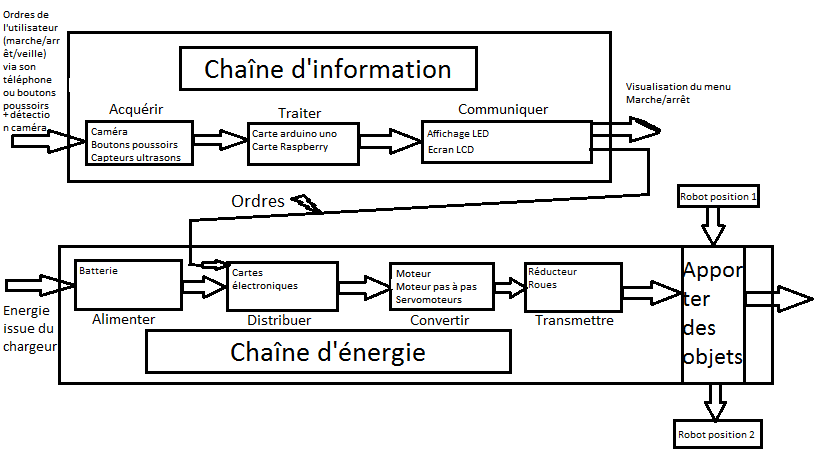
\includegraphics[width=145mm]{Diagramme_fonctionnel.png}
			\caption[Diagramme fonctionnel - Illustration réalisée par notre groupe, disponible à l'adresse : \url{https://github.com/thaspdev/PATRICK/illustrations/Diagramme_fonctionnel.png}]{Diagramme fonctionnel\label{overflow}}
	\end{figure}
	
Il nous a permis de représenter les différentes étapes du fonctionnement ; du repérage de l'utilisateur et de la réception de l'information par les cartes électroniques à la transmission du mouvement aux roues ; permettant le déplacement du robot d'une position 1 à une position 2.

Dans cette partie nous avons donc vu que le système souhaité peut être modélisé par différents diagrammes ayant tous un but particulier. A l'aide de ceux-ci nous avons pu trouver des solutions techniques adaptées aux contraintes et établir la liste des principaux composants. Il va donc désormais falloir sélectionner nos composants en fonction de leurs caractéristiques afin de respecter le cahier des charges.
	\newpage
	\section{Système simulé}
\indent \indent Après avoir identifié le besoin et trouvé les solutions techniques, il nous a fallu sélectionner nos pièces de manière plus précise avant de les commander. Nous les avons choisies pour que leurs caractéristiques répondent au cahier des charges. Dans cette partie nous avons décidé de séparer ces pièces en 2 catégories : mécanique et électronique.
	
	\subsection{Mécanique}
	
	\subsubsection{Système de direction}
	
\indent \indent Nous avons dans un premier temps réfléchi au système de direction. En effet le robot devait pouvoir orienter ses roues dans la direction de l’utilisateur de manière précise.
	
	\paragraph{Première version}\mbox{}\\

Le système auquel nous avons pensé dans un premier temps utilise seulement un moteur cc, un servomoteur, et une roue :

	\begin{figure}[ht!]
		\centering
			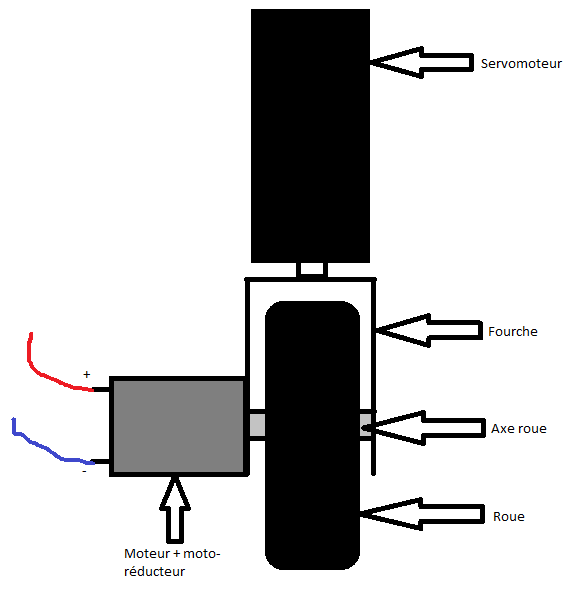
\includegraphics[width=90mm]{direction-face.png}
			\caption[Vue de face - Illustration réalisée par notre groupe, disponible à l'adresse : \url{https://github.com/thaspdev/PATRICK/illustrations/direction-face.png}]{Vue de face\label{overflow}}
	\end{figure}
	\begin{figure}[ht!]
		\centering
			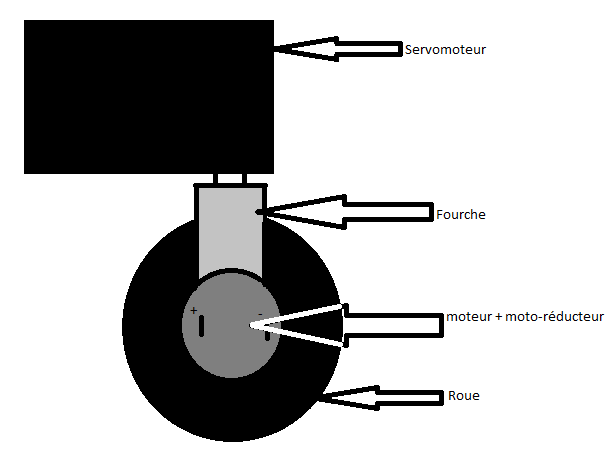
\includegraphics[width=80mm]{direction-profil.png}
			\caption[Vue de profil - Illustration réalisée par notre groupe, disponible à l'adresse : \url{https://github.com/thaspdev/PATRICK/illustrations/direction-profil.png}]{Vue de profil\label{overflow}}
	\end{figure}
	
	Ce système permet de faire tourner la roue et de l’orienter selon un angle bien précis effectué par le servomoteur :
	\begin{figure}[ht!]
		\centering
			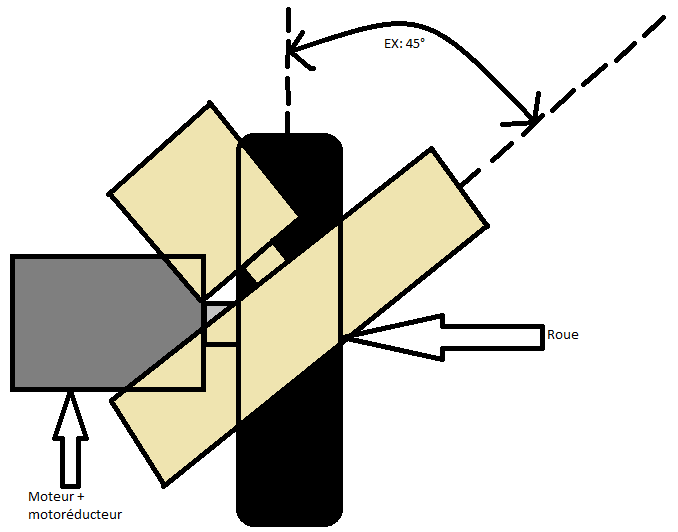
\includegraphics[width=120mm]{direction-dessous.png}
			\caption[Vue de dessous - Illustration réalisée par notre groupe, disponible à l'adresse : \url{https://github.com/thaspdev/PATRICK/illustrations/direction-dessous.png}]{Vue de dessous\label{overflow}}
	\end{figure}
	
	Seulement, ce système créait un problème de stabilité et de puissance. En effet si on avait utilisé ce système, le robot n’aurait reposé que sur ses trois roues folles et une seule roue motrice et sa tractation n’aurait été assurée que par cette unique roue motrice :
	
	\begin{figure}[ht!]
		\centering
			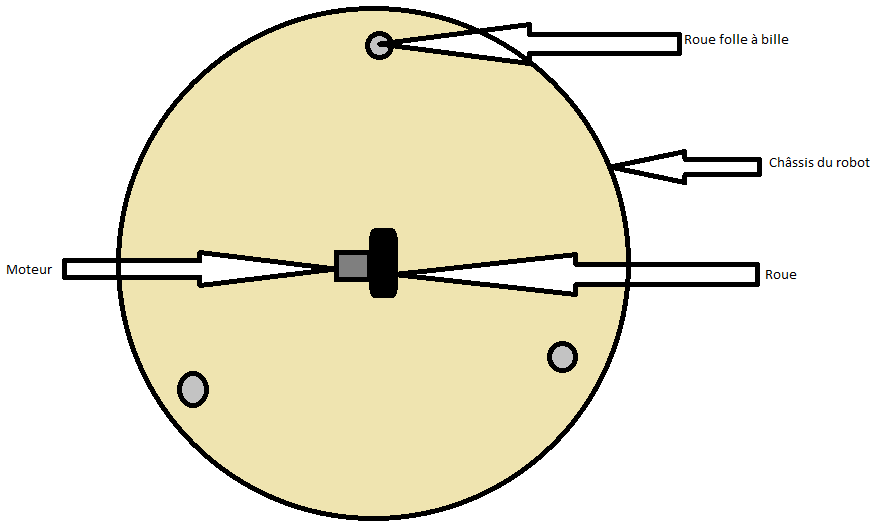
\includegraphics[width=130mm]{robot-dessous.png}
			\caption[Robot vu de dessous - Illustration réalisée par notre groupe, disponible à l'adresse : \url{https://github.com/thaspdev/PATRICK/illustrations/robot-dessous.png}]{Robot vu de dessous\label{overflow}}
	\end{figure}
	
	\begin{figure}[ht!]
		\centering
			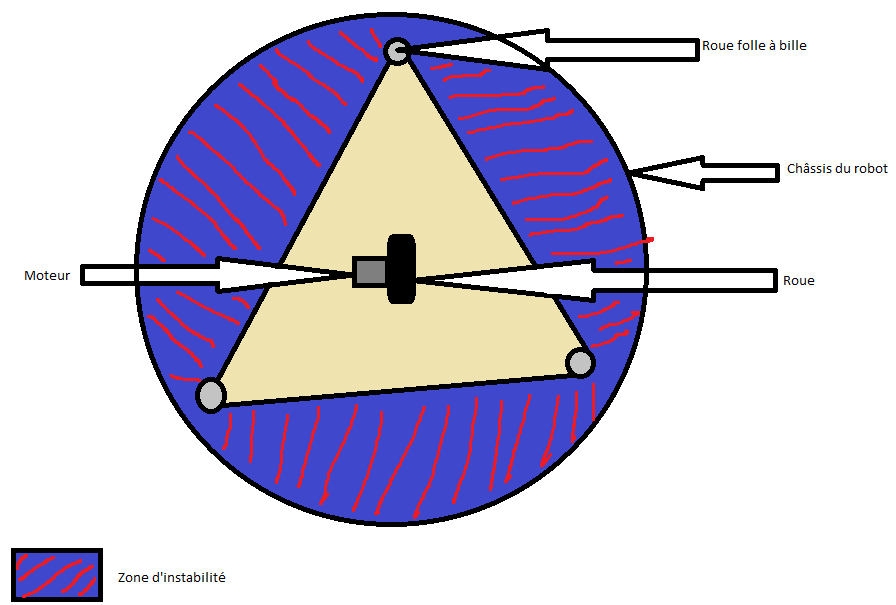
\includegraphics[width=130mm]{robot-instable.png}
			\caption[Robot vu de dessous avec la zone d'instablilité - Illustration réalisée par notre groupe, disponible à l'adresse : \url{https://github.com/thaspdev/PATRICK/illustrations/robot-instable.png}]{Robot vu de dessous avec la zone d'instablilité\label{overflow}}
	\end{figure}
	
	\paragraph{Réponse au problème de stabilité}\mbox{}\\
	
	Il y avait bien un problème de stabilité et de puissance motrice. De plus, la découpe du châssis aurait été tellement complexe à la scie à main ou onéreuse en magasin que nous avons finalement choisi un châssis carrée de 30cm de côté.
Pour remédier à ce problème de stabilité et de traction moteur, nous avons opté pour 4 quatre roues folles à bille et deux roues motrices.

	\begin{figure}[ht!]
		\centering
			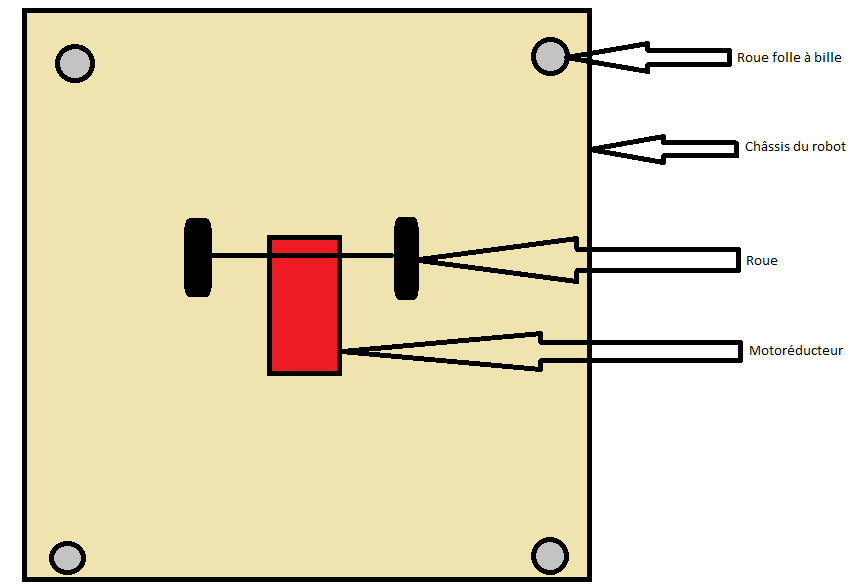
\includegraphics[width=130mm]{robot-final-dessous.png}
			\caption[Version finale du robot vu de dessous - Illustration réalisée par notre groupe, disponible à l'adresse : \url{https://github.com/thaspdev/PATRICK/illustrations/robot-final-dessous.png}]{Version finale du robot vu de dessous\label{overflow}}
	\end{figure}
	
	Mais l’utilisation de deux roue motrices implique que ces deux dernières soient retirées du sol avant que le servomoteur de direction de leur donne leur angle de rotation. Si ça n’avait pas été le cas, les roues aurait frotté sur le sol au moment de la rotation du servomoteur de direction et auraient contraint ce dernier à forcer pour vaincre ce frottement et ça l’aurait endommagé. Nous avons donc du utilisé un second servomoteur, permettant l’élévation des roues motrices et du motoréducteur.
	
	\begin{figure}[ht!]
		\centering
			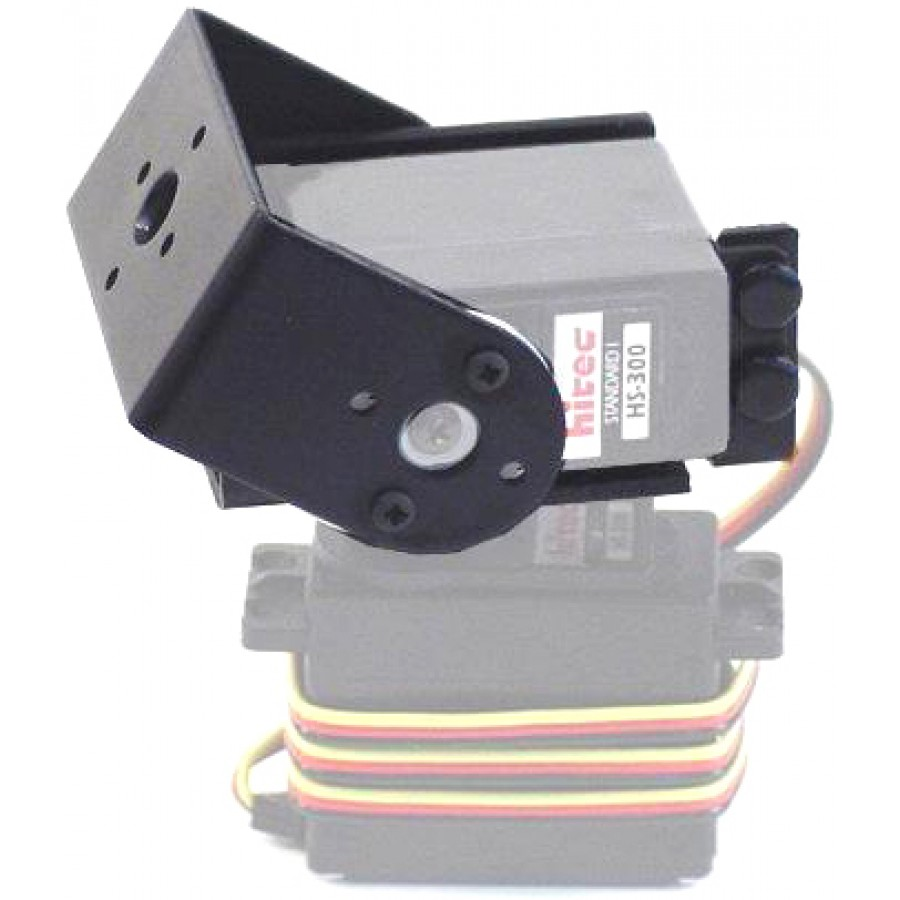
\includegraphics[width=60mm]{kit-aluminium-pan.jpg}
			\caption[Le kit tourelle que nous avons utilisé - Illustration provenant du site internet robotshop.com, disponible à l'adresse : \url{http://www.robotshop.com/eu/fr/kit-aluminium-pan-and-tilt-lynxmotion.html}]{Le kit tourelle que nous avons utilisé\label{overflow}}
	\end{figure}
	\newpage
	
	Nous avons donc utilisé un kit tourelle pour servomoteurs (lien dans la bibliographie).
	
	Nous avons ensuite choisi le motoréducteur pour qu'il soit capable de propulser le robot à une certaine vitesse :

	\subsubsection{Calcul du couple}
Avec la formule de la résistance au roulement nous avons calculé le couple qu'il devait développer pour la propulsion :
$$C_{\textit{nécessaire}} = \lambda \times m \times g + r \times F_{\textit{aéro}}+C_{\textit{résistant\_roue}}$$
Avec :

- $\lambda$ : coefficient de résistance au roulement = demie largeur de la zone de contact de la roue motrice avec le sol. En effet en fonction de la masse du véhicule et de sa matière, une roue à tendance à s'écraser légèrement, ce qui crée une adhérence et une force qui empêche le mouvement. (voir schéma)

	\begin{figure}[ht!]
		\centering
			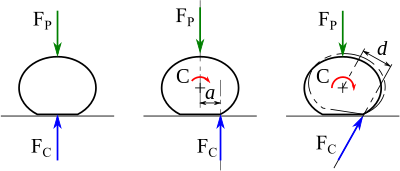
\includegraphics[width=80mm]{Resistance-roulement.png}
			\caption[Résistance au roulement d'une roue - Illustration publiée sous license GFDL (cf. Annexes) provenant de l'encyclopédie en ligne Wikipédia, disponible à l'adresse : \url{https://commons.wikimedia.org/wiki/File:Resistance_au_roulement_et_adherence_roue_motrice.svg}]{Résistance au roulement d'une roue\label{overflow}}
	\end{figure}
	
	Ici le coefficient est représenté par la distance $a$, et la force $F_p$ qui écrase la roue correspond au poids du véhicule ($m \times g$). Le couple $C$ correspond au couple nécessaire à vaincre cette force résistante d'où $C= a \times F_p$. On prendra  $\lambda = 0,0025$ pour notre pneu en caoutchouc de $\SI{36}{ \milli\meter}$ de diamètre.

- $m$ : masse du robot chargé : $\SI{10}{\kilogram}$

- $g$ : gravité terrestre : $9,81 \text{ }\SI{}{\meter}\cdot\SI{}{\per\second\squared}$

- $r$ : rayon de la roue motrice : $\SI{18}{\milli\meter}$

- Force résistante aérodynamique : force qui empêche le mouvement d'un objet dans l'air $F_{\textit{aéro}} = \dfrac{1}{2} \times \rho_{air} \times v^2 \times C_x \times S$ avec :\\
\indent \indent - $\rho_{air}$ : masse volumique de l'air : $1,225 \text{ }\SI{}{\kilogram}\cdot\SI{}{\per\meter\cubed}$\\
\indent \indent - $v^2$ :vitesse au carré : $0,5\times 0,5 \text{ }\SI{}{\meter} \cdot \SI{}{\per\second}$ (cahier des charges)\\
\indent \indent - $C_x$ : coefficient de trainée en fonction de la forme : $1,05$ (cube)
	\begin{figure}[ht!]
		\centering
			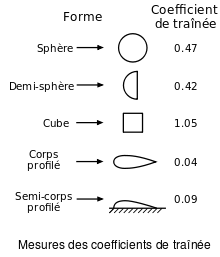
\includegraphics[width=70mm]{Coeff-trainee.png}
			\caption[Coefficient de trainée en fonction de la forme - Illustration du domaine public provenant de l'encyclopédie en ligne Wikipédia, disponible à l'adresse : \url{https://commons.wikimedia.org/wiki/File:Drag-fr.svg}]{Coefficient de trainée en fonction de la forme\label{overflow}}
	\end{figure}
	
\indent \indent - $S$ : surface de contact (face du robot) : $0,09 \SI{}{\meter\squared}$ 
donc $F_{\textit{aéro}} = \dfrac{1}{2} \times 1,225 \times 0,5 \times 0,5 \times 1,05 \times 0,09 = 0,015 \text{ } \SI{}{\newton}$
	
-Couple résistant roue : couple nécessaire à faire tourner la roue dans le vide (négligeable)
 
Donc Couple nécessaire = 0,0025*10*9,81+0,018*0,015 = 0,2455 N.m

\subsubsection{Calcul de la vitesse de rotation de la roue souhaitée}
\begin{align*}
N_{roue} &= \dfrac{Vitesse}{\textit{Périmètre de la roue}} = \dfrac{0,536}{\pi \times 0,001}\\
\Leftrightarrow N_{roue} &= 4,4 \text{ tr}\cdot\SI{}{\per\second} = 258 \text{ tr} \cdot \SI{}{\per\minute} = 27 \text{ } \SI{}{\radian} \cdot \SI{}{\per\second}
\end{align*}

\subsubsection{Calcul de la puissance du motoréducteur à acheter}
$$P = C \cdot \omega = 0,2455 \times 27 = 6,8 \text{ } \SI{}{\watt}$$

Ces calculs nous ont donc permis d'acheter le moteur qui convient.
	
	\subsection{Électronique}
	\indent\indent Dans cette partie, nous traiterons du système électronique simulé du robot.
	
	\subsubsection{Écran LCD et boutons poussoirs}
	
\indent\indent Afin d’établir la communication entre le robot et l’utilisateur nous avons fait le choix d’utiliser un écran LCD (liquid crystal display ou affichage à cristaux liquides). Il permet un affichage simple à faible consommation d’électricité. L’écran LCD est passif, c’est-à-dire qu’il n’émet pas de lumière ; seule la transparence de ses caractères peut varier et pour cela nous utilisons un potentiomètre. Afin que ce qu’il affiche soit lisible, il admet un rétro-éclairage effectué par une LED (diode électroluminescente). 

En sachant que l’alimentation de cette LED est assurée par un Arduino de tension $\SI{5}{\volt}$ et de courant $\SI{23}{\milli\ampere}$ nous avons déterminé la résistance à placer dans notre câblage. La loi d’Ohm nous permet de poser la relation suivante \nolinebreak: $U = R\cdot I$, avec $U$ pour la tension en Volts, $I$ le courant en Ampères et $R$ la résistance en Ohms.

	\begin{align*}
		U &= R\cdot I\\
		R &= \dfrac{U}{I}\\
		R &=  \dfrac{5}{0,023}\\
		R &= \SI{217}{\ohm}
	\end{align*}
	
	Nous avons donc sélectionné une résistance dont la valeur se rapprochait le plus de ce résultat, c’est-à-dire $\SI{220}{\ohm}$.

Cet écran affiche un menu commandé par plusieurs interrupteurs \nolinebreak : des boutons poussoirs. Ils permettent d’ouvrir et de fermer un circuit alimentant un appareil électrique. Ceux-ci sont branchés en "pull-down resistor".
Dans un montage de résistance pull-down, une résistance supplémentaire de $\SI{10}{\kilo\ohm}$ est utilisée pour amener l’entrée à la masse et cela permet de limiter les rebonds (interférences pouvant gêner le bon fonctionnement du programme) lors de l’utilisation.

	\begin{figure}[ht!]
		\centering
			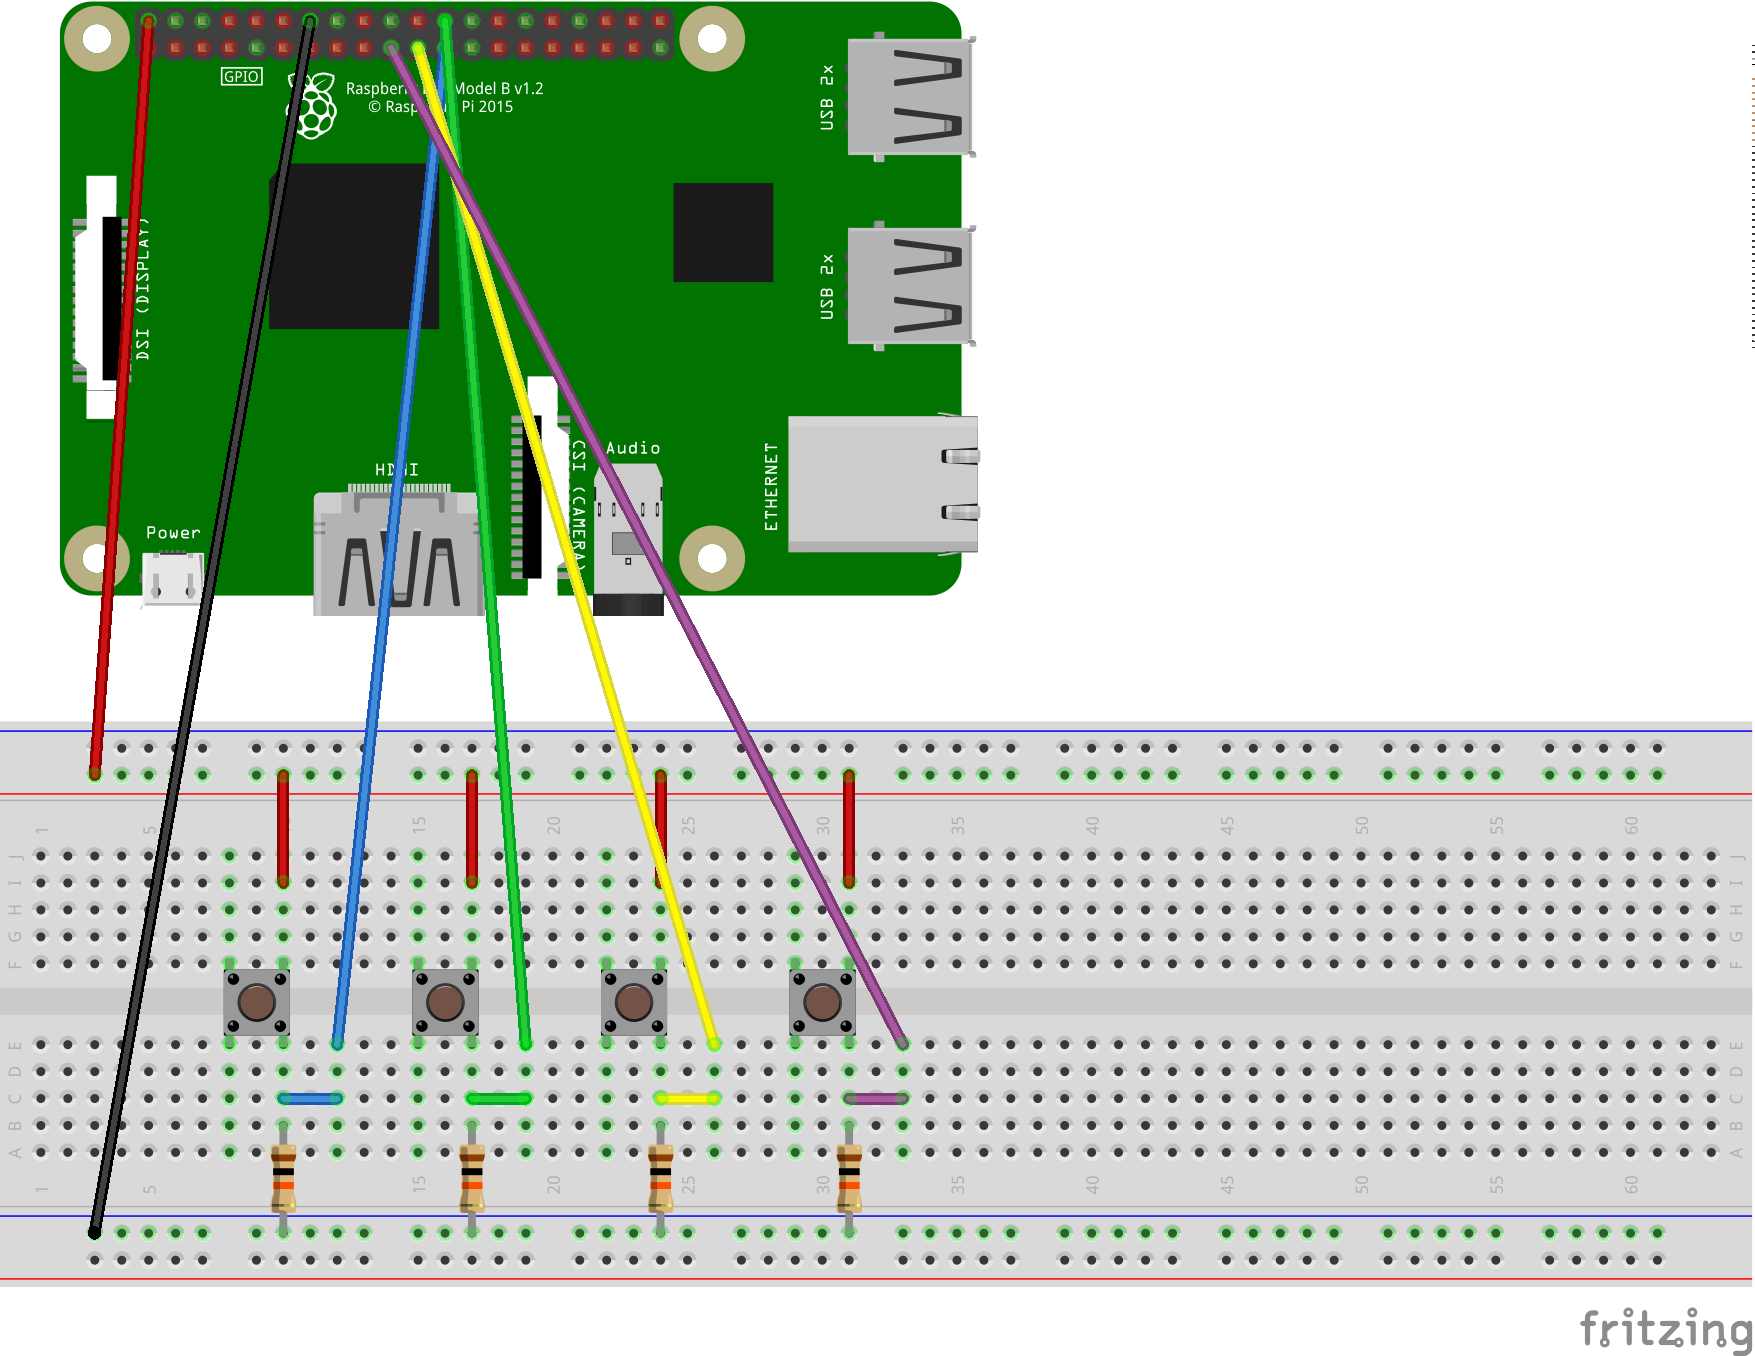
\includegraphics[width=140mm]{Raspi_poussoir_bb.png}
			\caption[Schéma du câblage des boutons poussoirs - Illustration réalisée par notre groupe, disponible à l'adresse : \url{https://github.com/thaspdev/PATRICK/blob/master/circuits/Raspi_poussoir/Raspi_poussoir_bb.png}, ainsi qu'à cette adresse au format Fritzing : \url{https://github.com/thaspdev/PATRICK/blob/master/circuits/Raspi_poussoir/Raspi_poussoir.fzz}]{Schéma du câblage des boutons poussoirs\label{overflow}}
	\end{figure}
	
	\begin{figure}[ht!]
		\centering
			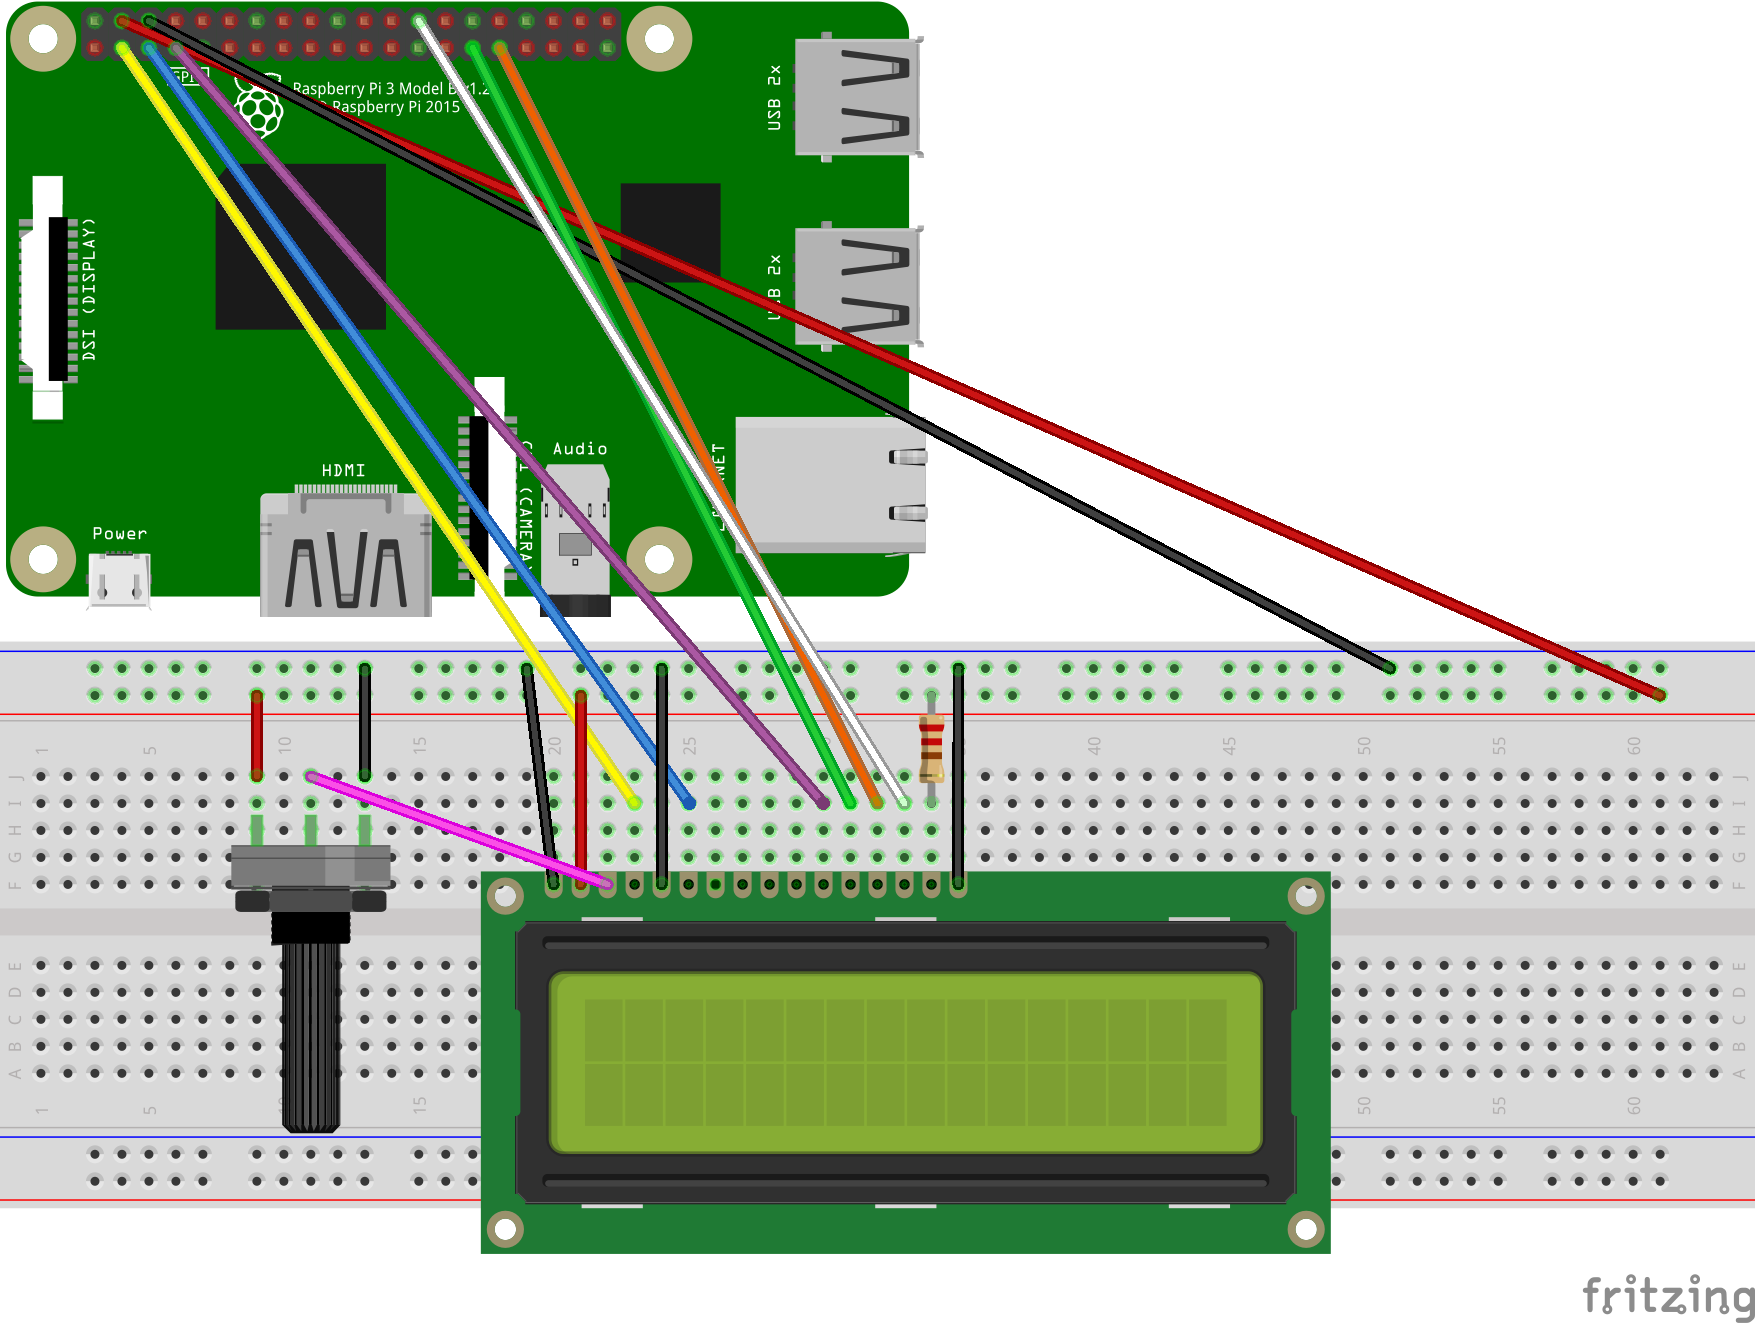
\includegraphics[width=140mm]{Raspi_lcd_bb.png}
			\caption[Schéma du câblage de l'écran LCD - Illustration réalisée par notre groupe, disponible à l'adresse : \url{https://github.com/thaspdev/PATRICK/blob/master/circuits/Raspi_lcd/Raspi_lcd_bb.png}, ainsi qu'à cette adresse au format Fritzing : \url{https://github.com/thaspdev/PATRICK/blob/master/circuits/Raspi_lcd/Raspi_lcd.fzz}]{Schéma du câblage de l'écran LCD\label{overflow}}
	\end{figure}
	\newpage
	
	\subsubsection{Moteur à courant continu}
	
	Pour répondre à la fonction "se déplacer" (FT4), le robot utilise un moteur à courant continu, alimenté en $\SI{18}{\volt}$ et $0,3 \text{ } \SI{}{\ampere}$. Pour le piloter, nous utilisons un driver moteur L293D.
	
	\begin{figure}[ht!]
		\centering
			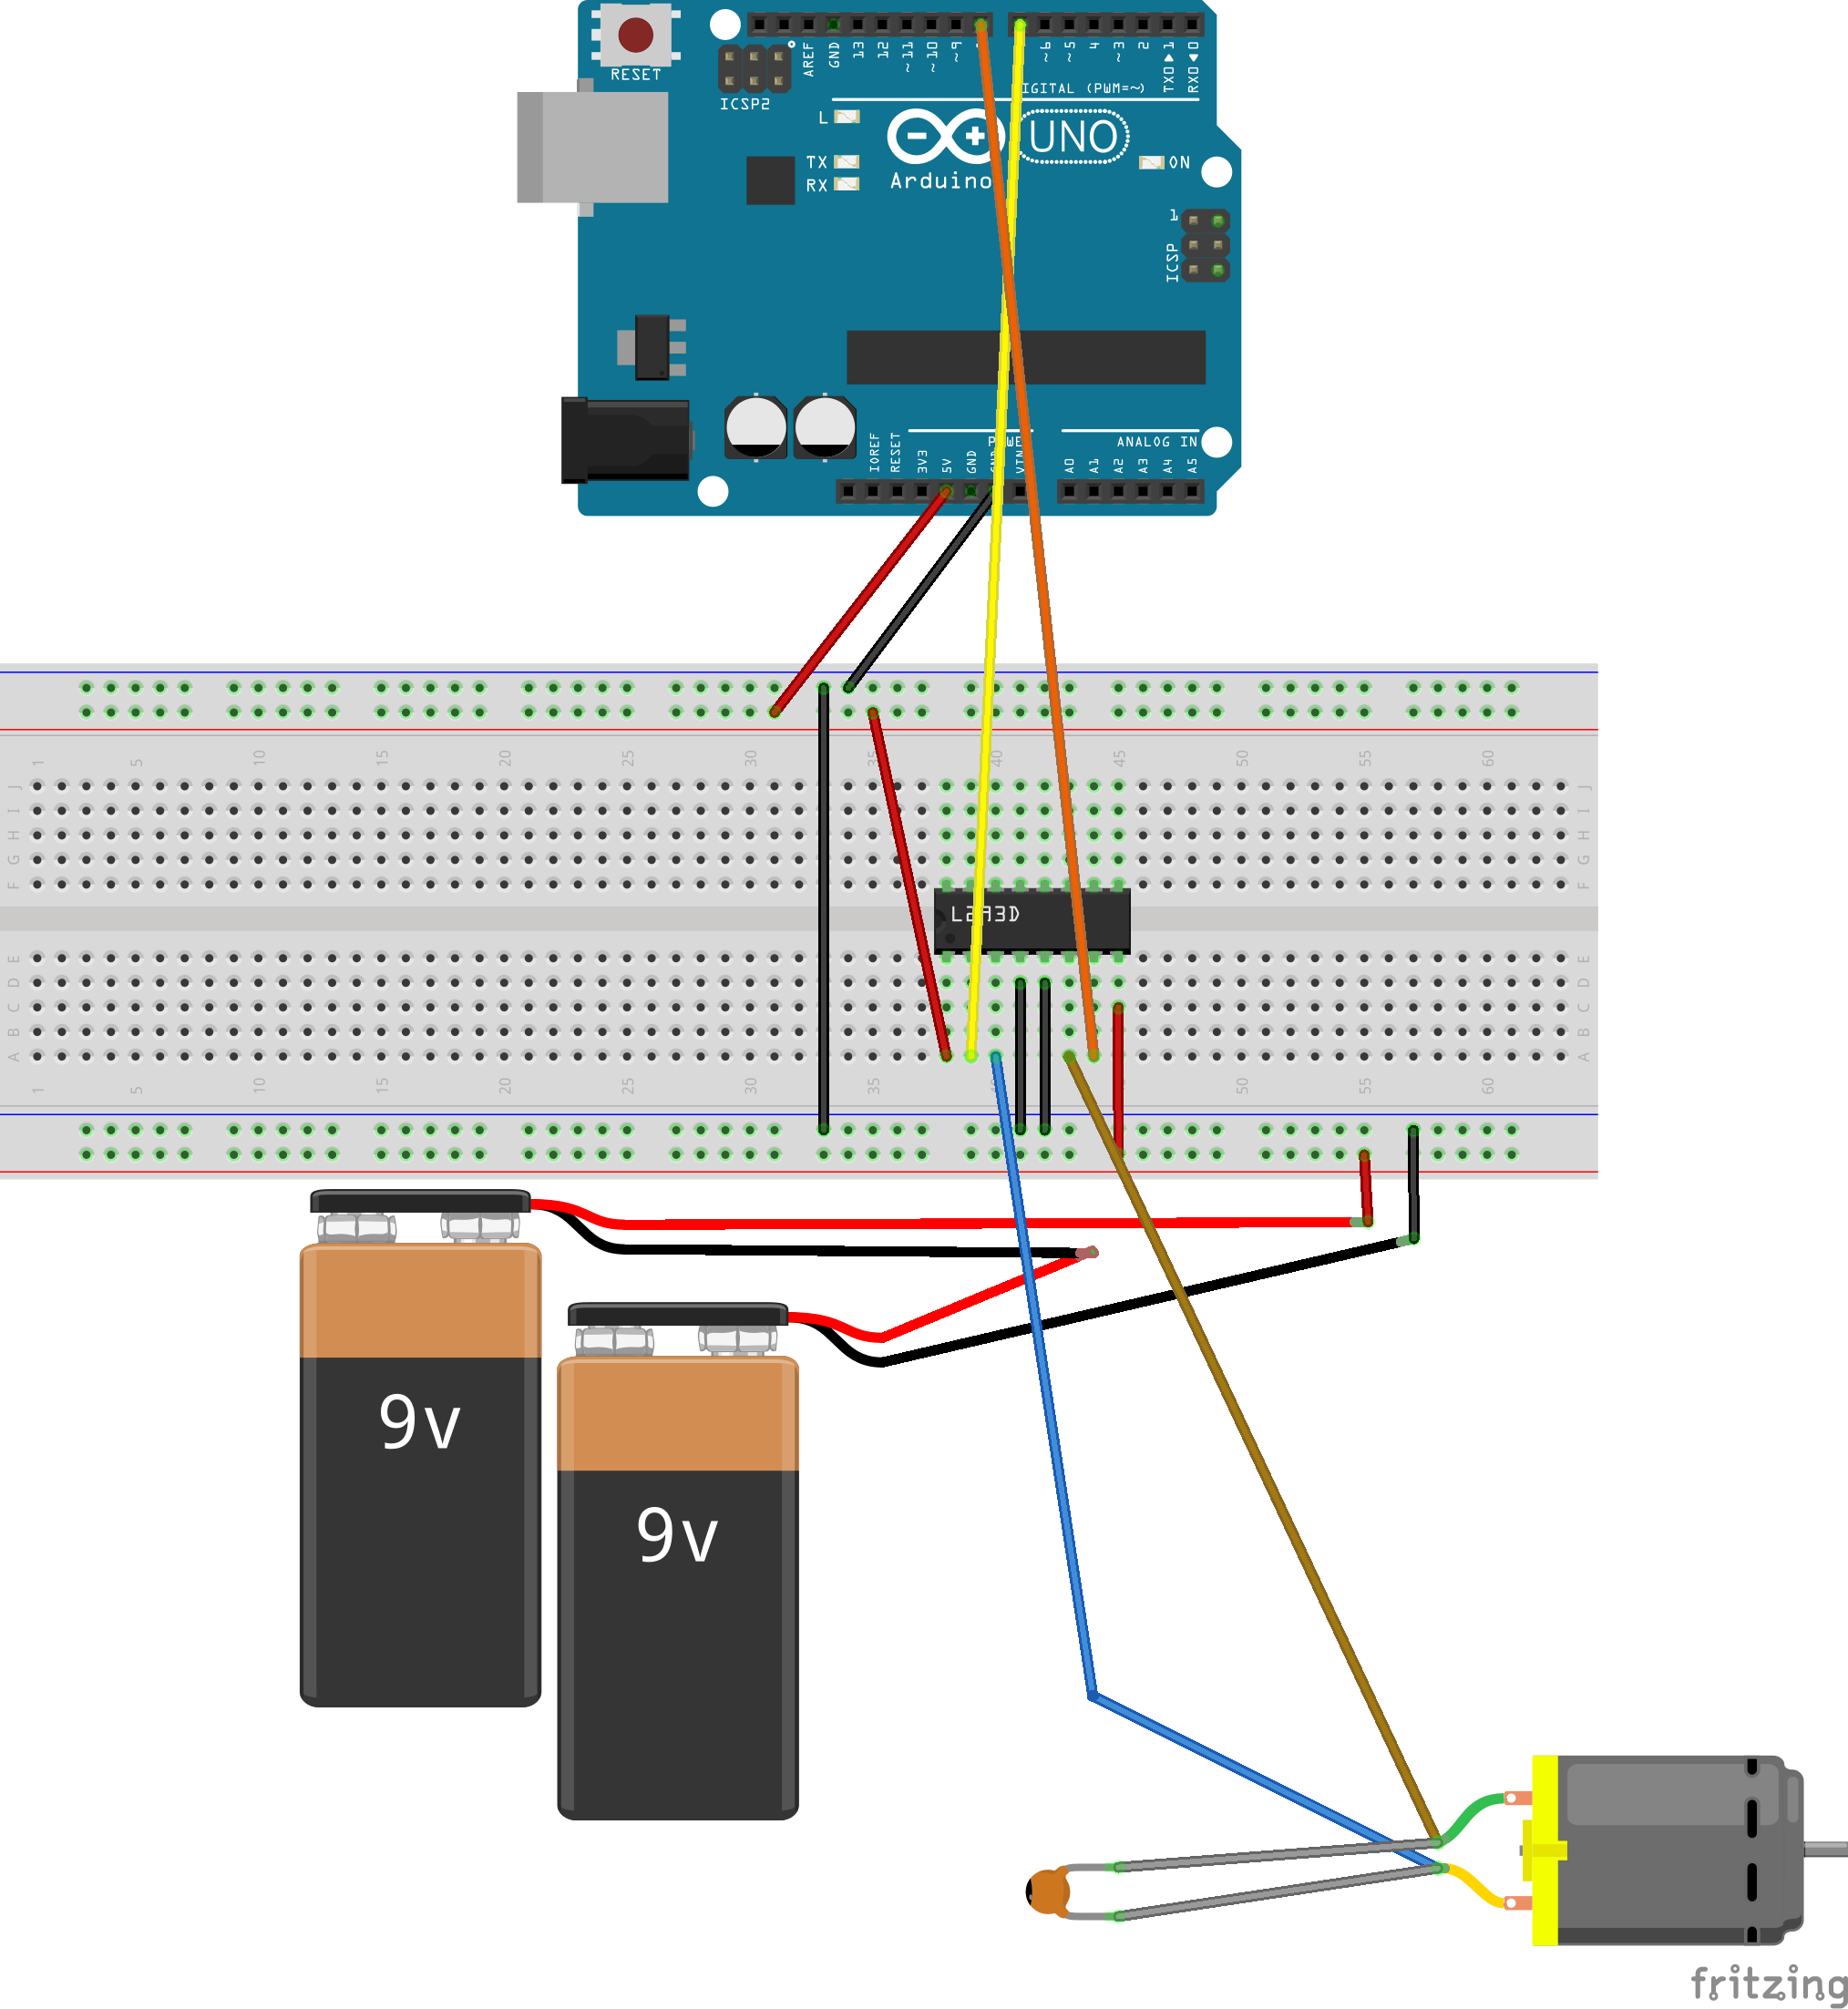
\includegraphics[width=140mm]{Arduino_moteur_bb.png}
			\caption[Schéma du câblage du moteur à courant continu - Illustration réalisée par notre groupe, disponible à l'adresse : \url{https://github.com/thaspdev/PATRICK/blob/master/circuits/Arduino_moteur/Arduino_moteur_bb.png}, ainsi qu'à cette adresse au format Fritzing : \url{https://github.com/thaspdev/PATRICK/blob/master/circuits/Arduino_moteur/Arduino_moteur.fzz}]{Schéma du câblage du moteur à courant continu\label{overflow}}
	\end{figure}
	\newpage
	
	Le L293D est aussi connu pour être une sorte de pont en H. Un pont en H est un circuit électrique qui permet de contrôler la polarité aux bornes d’un dipôle. Dans notre cas il s’agit d’un moteur à courant continu.
En changeant la polarité, le pont en H permet donc de changer le sens de rotation du moteur.
Le driver fonctionne avec une source de tension venant de la carte Arduino égale à $\SI{5}{\volt}$.
Une diode de roue libre est intégrée dans le montage afin de protéger la carte Arduino lorsqu’on coupe le courant alimentant le moteur.

\subsubsection{Moteur pas à pas}

\begin{figure}[ht!]
		\centering
			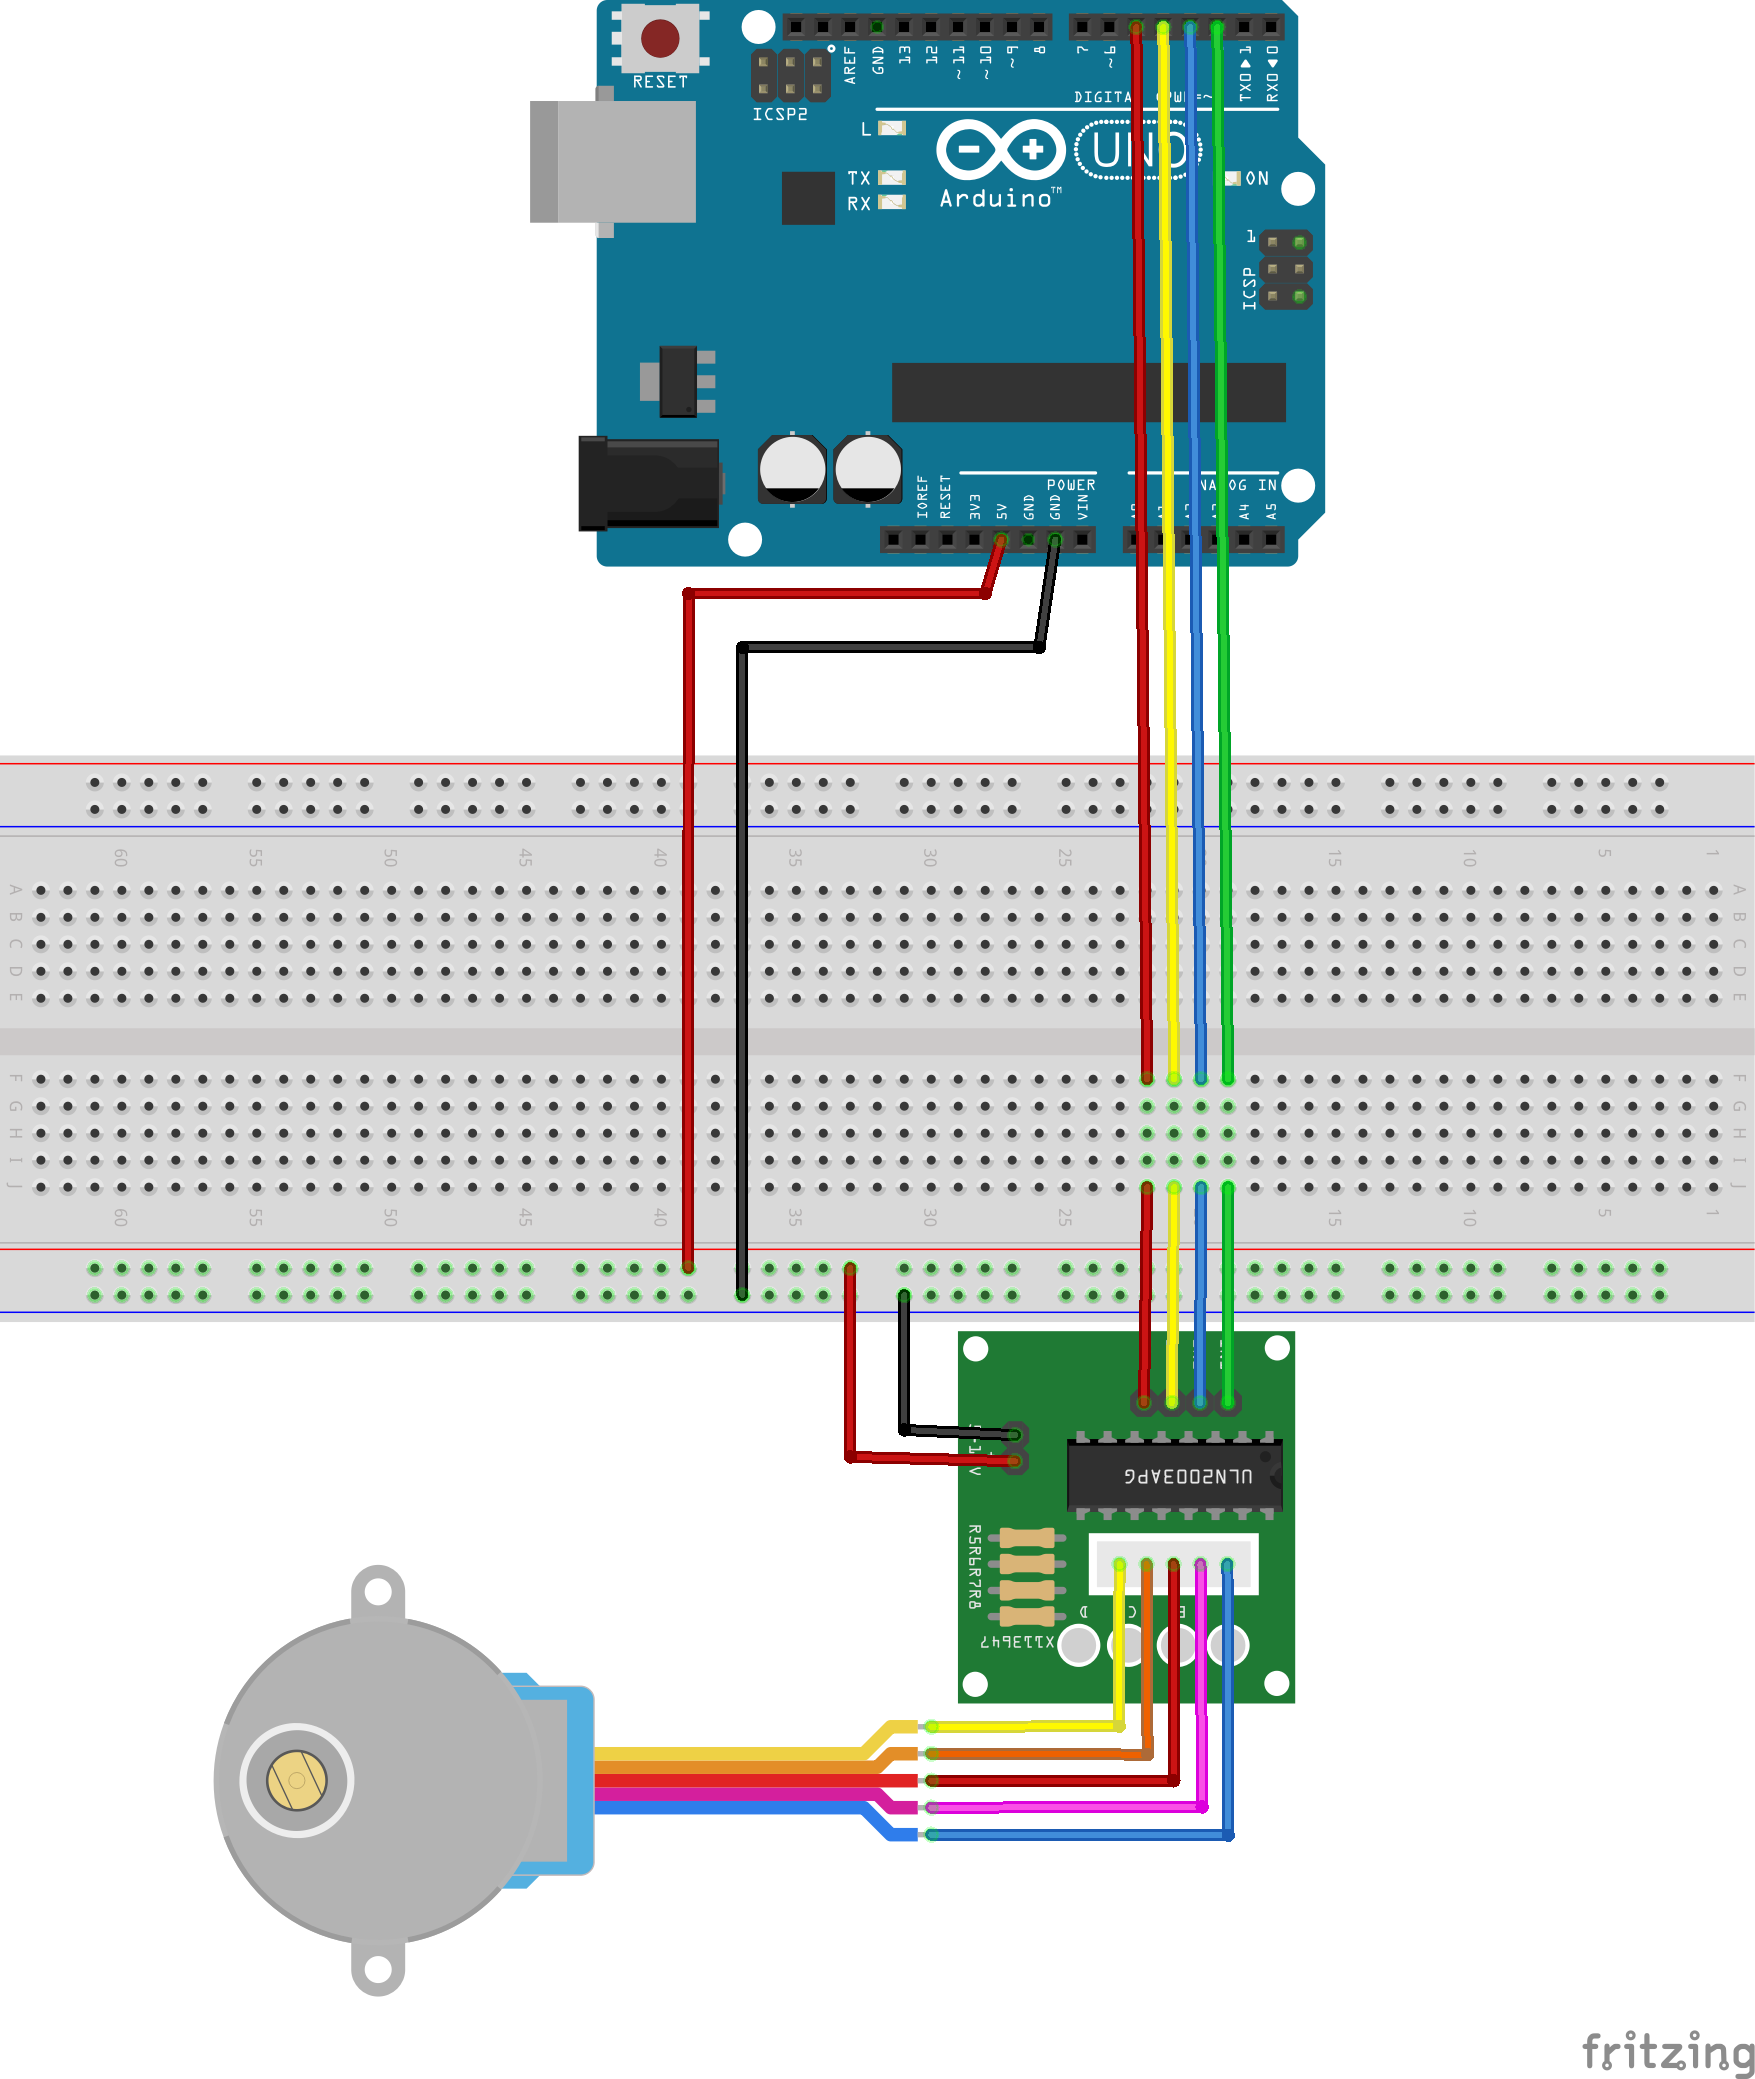
\includegraphics[width=140mm]{Arduino_stepper_bb.png}
			\caption[Schéma du câblage du moteur pas à pas - Illustration réalisée par notre groupe, disponible à l'adresse : \url{https://github.com/thaspdev/PATRICK/blob/master/circuits/Arduino_stepper/Arduino_stepper_bb.png}, ainsi qu'à cette adresse au format Fritzing : \url{https://github.com/thaspdev/PATRICK/blob/master/circuits/Arduino_stepper/Arduino_stepper.fzz}]{Schéma du câblage du moteur pas à pas\label{overflow}}
	\end{figure}

Pour assurer la rotation à $360 ^\circ$ de la caméra nous utilisons un moteur pas à pas. La fonction de ce moteur pas à pas est de contrôler la vitesse et la position du système mécanique souhaité : ici la caméra. En effet nous avons besoin de réguler la vitesse de rotation de la caméra ainsi que relever l’angle de perception d’un visage grâce à la connaissance de position prise par le moteur pas à pas. Il possède également un driver propre à lui-même qui le pilote de manière à connaître son pas et transmettre l’information à l’Arduino.

\subsubsection{Servomoteur}

Ce type de moteur rassemble deux parties qui fonctionnent de pair pour assurer une fonction finale commune :

Une partie mécanique composé d’un moteur à courant continu de petite taille, d’un réducteur en sortie de ce moteur permettant de diminuer la vitesse et donc d’augmenter le couple et d’un axe dépassant hors du boîtier avec différents bras de fixation. 
Ainsi qu’une partie électrique qui regroupe un dispositif électrique d’asservissement qui joue sur la partie mécanique. En effet les signaux électriques imposent au moteur un ordre pour que l’axe de sortie soit conforme à l’angle souhaité. Et un potentiomètre qui génère une tension variable, proportionnelle à l’angle pris par l’axe de sortie.

Les servomoteurs servent à actionner les parties mobiles d’un système de manière précise. Les servomoteurs sont commandés par l’intermédiaire d’un câble électrique à trois fils qui permet d’alimenter le moteur et de lui transmettre des consignes de position sous forme de signaux continus. On appelle cette technique la modulation par largeur d’impulsions (MLI). Celle-ci consiste à traduire des signaux électriques en information de position pour l’axe de sortie. Lorsque le moteur tourne, l’axe du servomoteur change de position, ce qui modifie la résistance du potentiomètre. Le rôle de l’électronique est de commander le moteur pour que la position de l’axe de sortie soit conforme à la consigne reçue : il s’agit donc d’asservissement. L’angle qui lui est imposé vient du Raspberry Pi.
Dans notre cas la tourelle servomoteur permet d’assurer l’élévation temporaire des roues motrices afin que le second servomoteur, en charge de la direction, permette d’assurer la rotation de celles-ci.

	\begin{figure}[ht!]
		\centering
			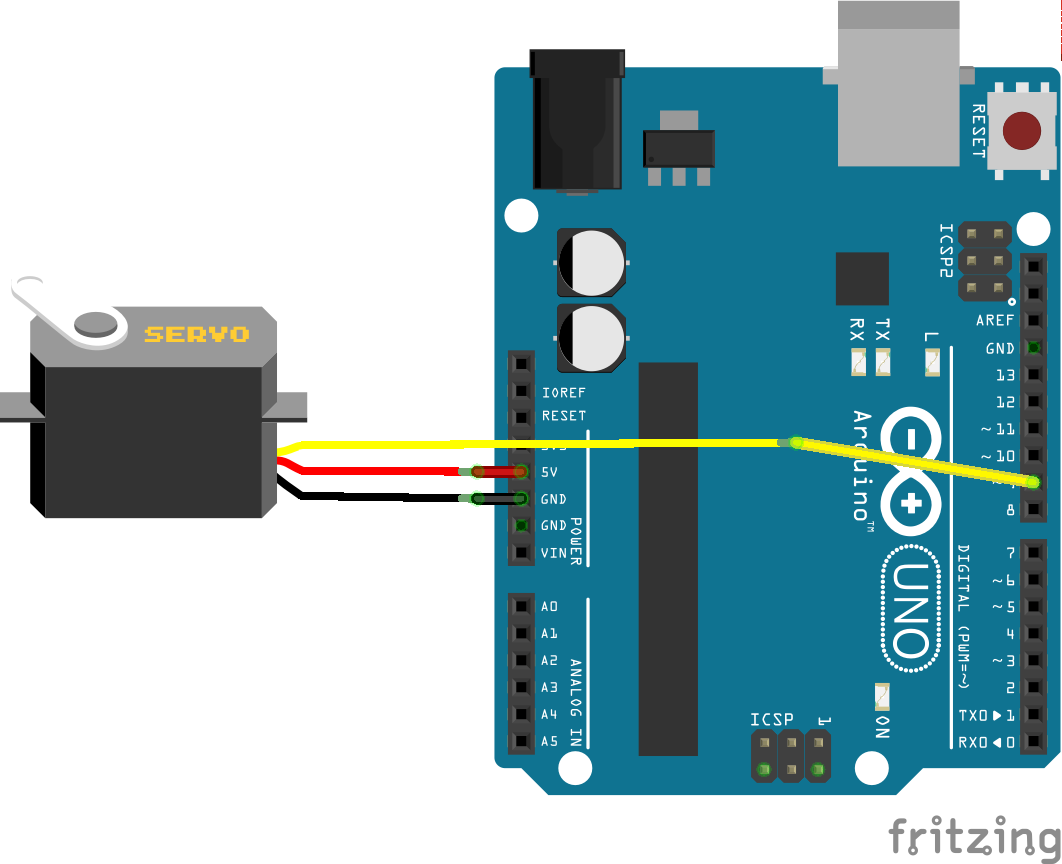
\includegraphics[width=140mm]{Arduino_servo_bb.png}
			\caption[Schéma du câblage d'un des servomoteurs - Illustration réalisée par notre groupe, disponible à l'adresse : \url{https://github.com/thaspdev/PATRICK/blob/master/circuits/Arduino_servo/Arduino_servo_bb.png}, ainsi qu'à cette adresse au format Fritzing : \url{https://github.com/thaspdev/PATRICK/blob/master/circuits/Arduino_servo/Arduino_servo.fzz}]{Schéma du câblage d'un des servomoteurs\label{overflow}}
	\end{figure}
	\newpage
	
	Ensuite, le robot permet de visualiser un visage autour de lui dans un rayon d’au moins 5 mètres. Cette fonction est assurée par une caméra spécifique au Raspberry Pi (également utilisée dans des téléphones portables) dont l’angle de vision est égal à $62,2^\circ$. Grâce au programme réalisé, elle permet de reconnaître les visages humains. Cette caméra est alimentée par le Raspberry Pi en $\SI{5}{\volt}$. Elle est branchée par une nappe de câble a un port spécial conçu à cet effet sur ce dernier. Quand la caméra repère une personne, le Raspberry Pi transmet à l’Arduino l’angle auquel cette dernière se trouve, afin que celui-ci l’impose au servomoteur de direction pour que le robot se dirige vers la personne aperçue.
	
	\begin{figure}[ht!]
		\centering
			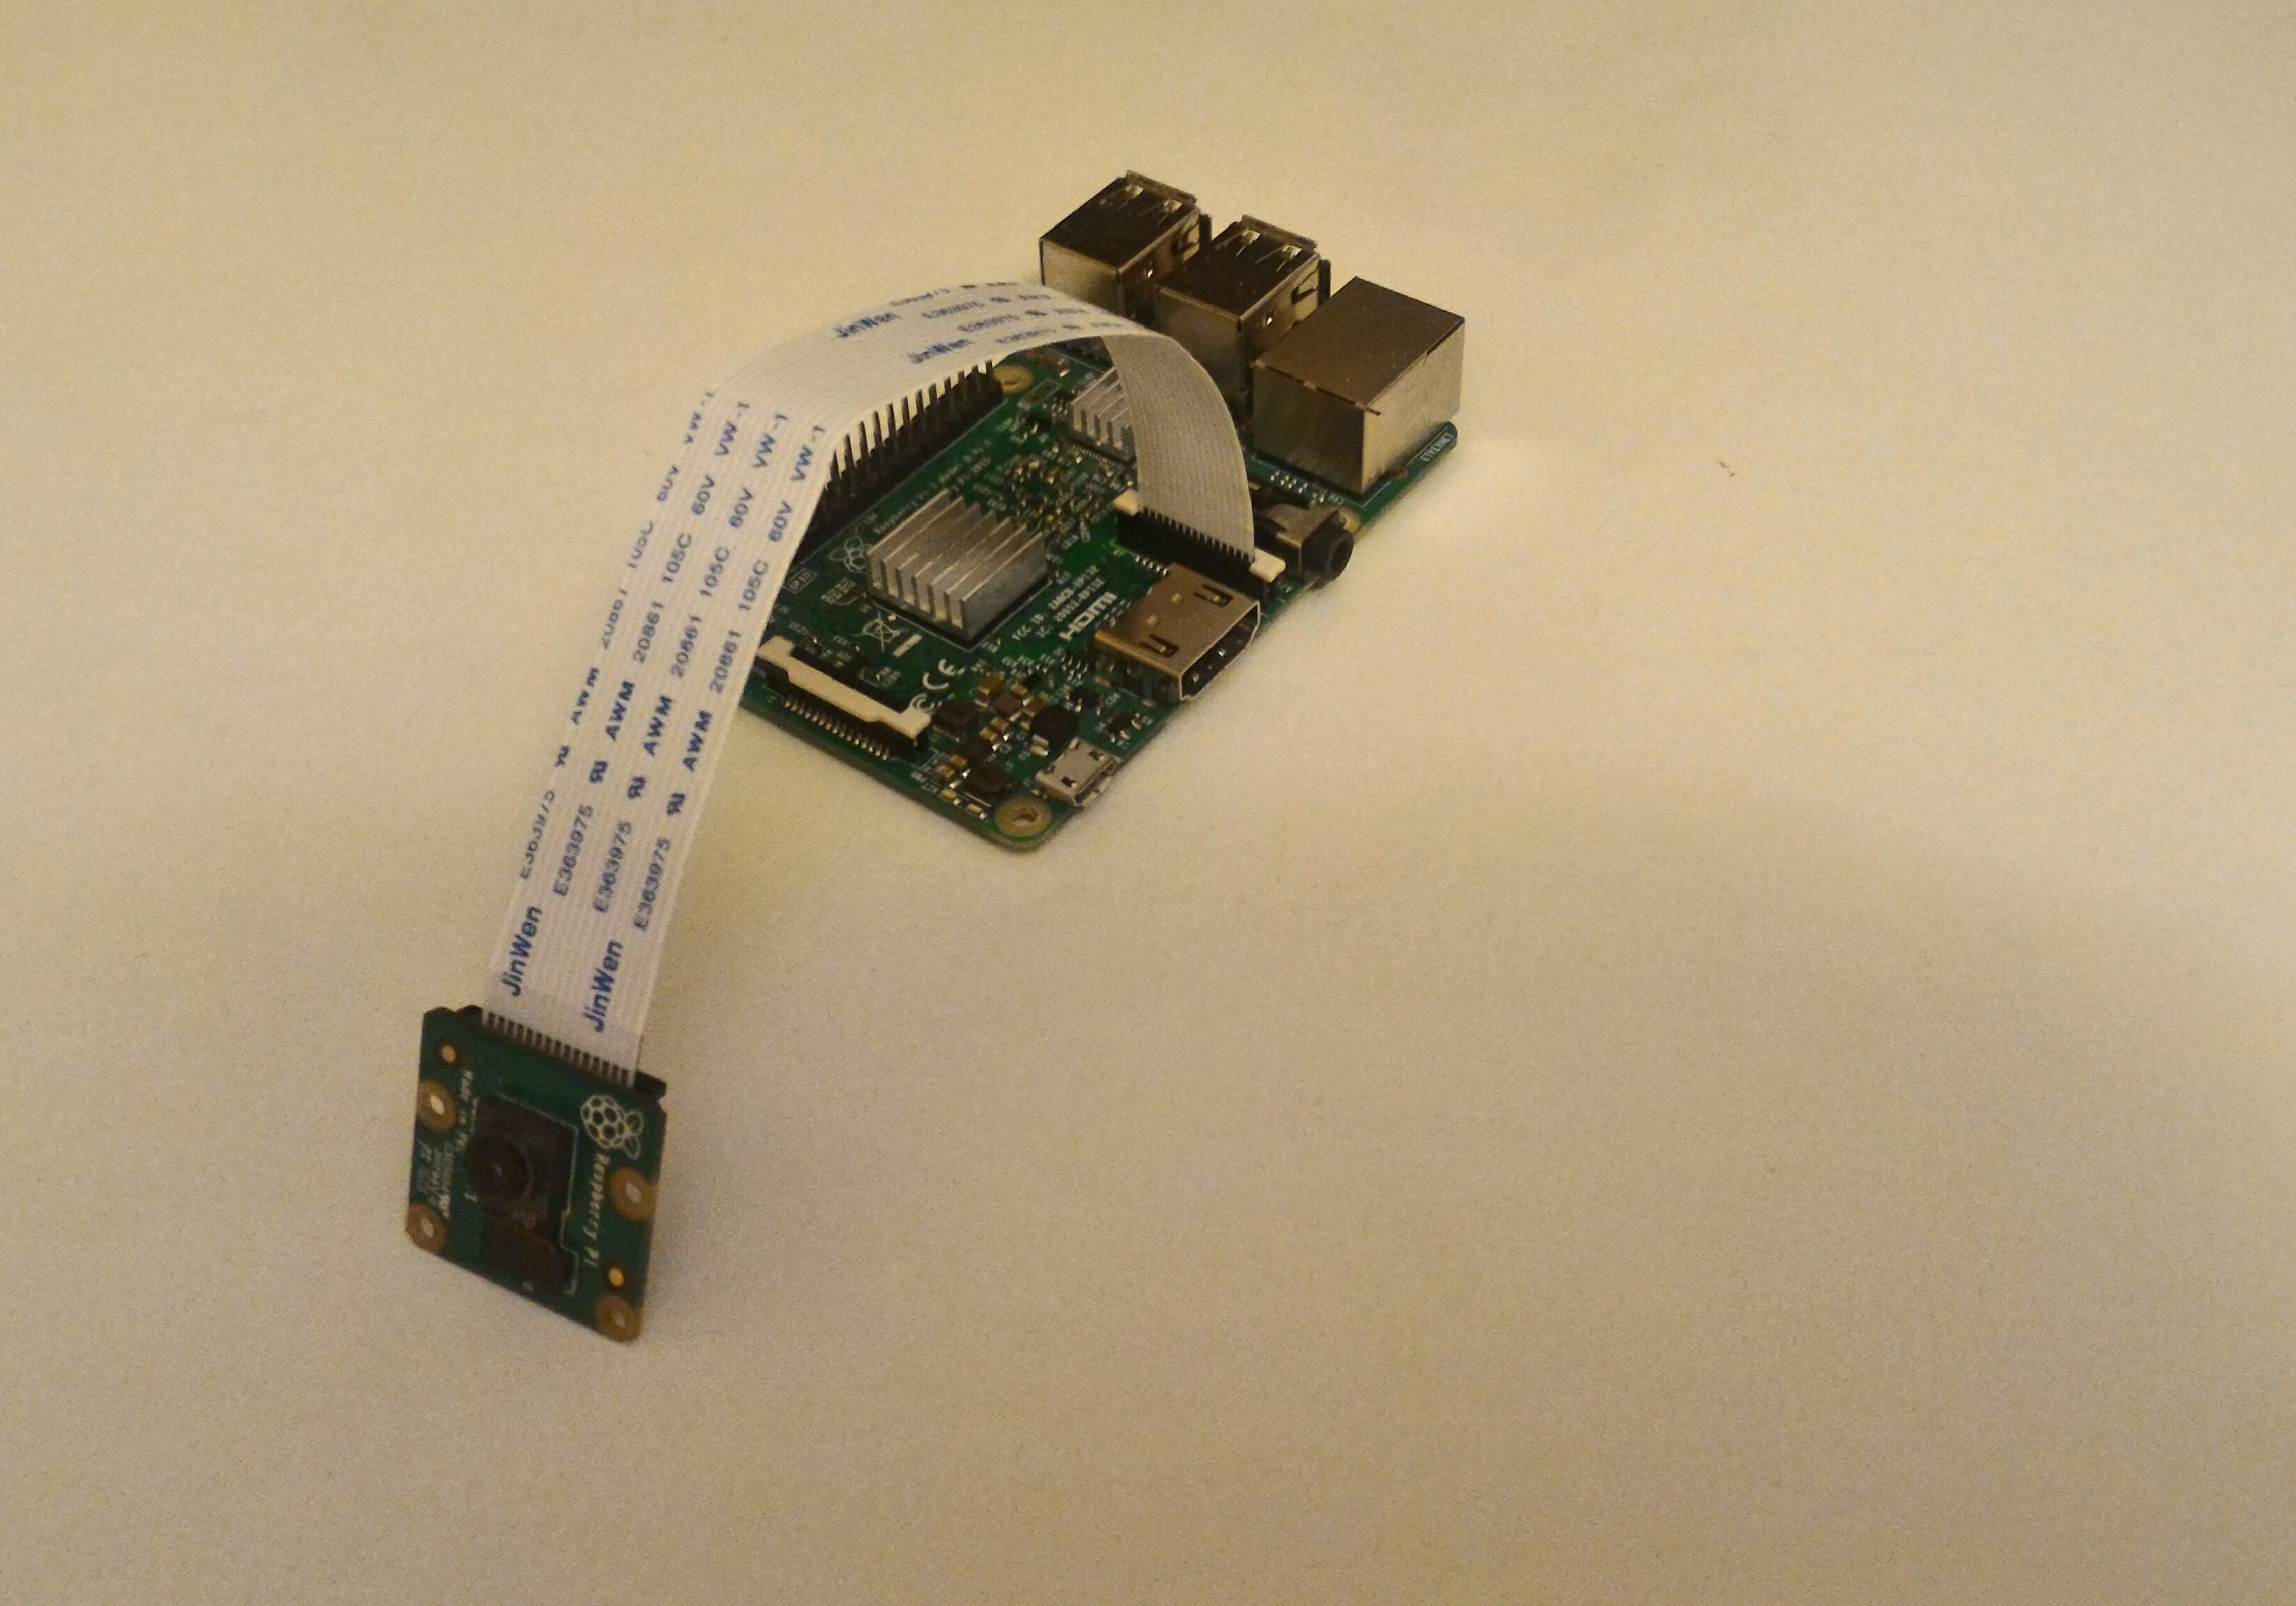
\includegraphics[width=140mm]{Raspi_camera.jpg}
			\caption[Schéma du câblage du moteur à courant continu - Illustration réalisée par notre groupe, disponible à l'adresse : \url{https://github.com/thaspdev/PATRICK/blob/master/illustrations/Raspi_camera.jpg}]{Le Raspberry Pi et la caméra l'accompagnant\label{overflow}}
	\end{figure}
	\newpage
	
	Le système est entièrement alimenté par une batterie de $\SI{5}{\volt}$ qui délivre un courant de $2,1\text{ } \SI{}{\ampere}$. Nous avons choisi de produire cette tension pour s’adapter à ce que nécessite le Raspberry Pi pour fonctionner correctement. L’Arduino fonctionne par une prise USB qui le relie au Raspberry pour lui délivrer une tension de $\SI{5}{\volt}$.
	\newpage
	\section{Système réel}
	
	\subsection{Construction du robot}
	
	Après avoir complété toute la partie sur le système simulé, nous avons commencé à nous atteler à la construction même du robot.
	
	\subsubsection{Construction du corps}
	
\indent\indent Dans un premier temps, le robot devait avoir un forme cylindrique. Seulement, le prix et la complexité de la découpe nous ont forcé à revoir le cahier des charges. Nous avons donc opté pour une forme plus simple et moins coûteuse. Le robot aura donc une forme parallélépipédique : il contiendra une base carrée de 30 cm de côté et 40 cm de hauteur :
	
	\begin{figure}[ht!]
		\centering
			\includegraphics[width=140mm]{Schema_construction_corps_modifie.png}
			\caption{Schéma du corps du robot\label{overflow}}
	\end{figure}
	
	Par conséquent la découpe a été plus simple et l’assemblage également :
	
	\begin{figure}[ht!]
		\centering
			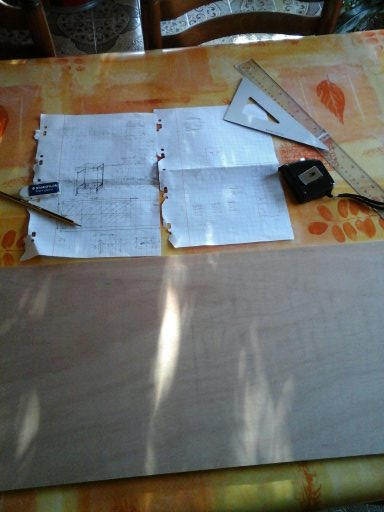
\includegraphics[width=60mm]{Planche_avant_decoupe.jpg}
			\caption{Planche ayant servi à la construction du robot\label{overflow}}
	\end{figure}
	\newpage
	
	Pour la découpe nous avons utilisé une scie à ruban :
	
	\begin{figure}[ht!]
		\centering
			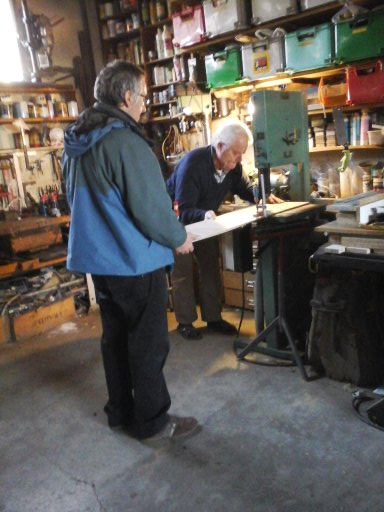
\includegraphics[width=61mm]{Decoupe_planche_scie_ruban.jpg}
			\caption{Découpe du robot à la scie à rubans\label{overflow}}
	\end{figure}
	
	Le montage en lui-même fut très long et nous dûmes à plusieurs reprises recoller les pans, car la colle à bois à un temps de séchage plutôt long.
Après avoir percé le trou pour la caméra, celui pour l’écran LCD et ceux pour les boutons poussoirs, nous nous avons pu assembler toutes les parties composant le corps du robot et voici le résultat final :

	\begin{figure}[ht!]
		\centering
			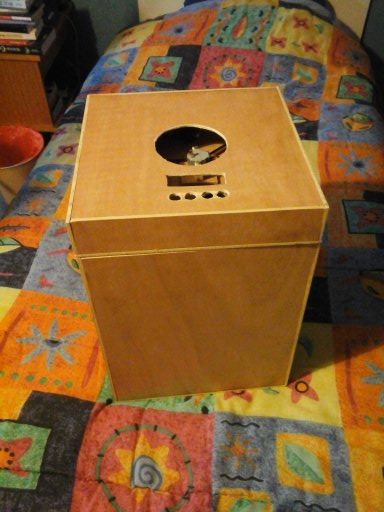
\includegraphics[width=48mm]{Robot_decoupe_perce.jpg}
			\caption{Robot après la découpe, l'assemblage et le perçage\label{overflow}}
	\end{figure}
	
	\begin{figure}[ht!]
		\centering
			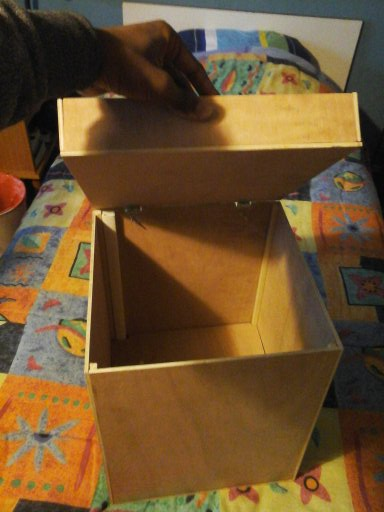
\includegraphics[width=48mm]{Robot_decoupe_ouvert.jpg}
			\caption{Robot ouvert après la découpe, l'assemblage et le perçage\label{overflow}}
	\end{figure}
	
	Après avoir terminé cette partie de la construction, il fallut passer au câblage électronique. Le programme étant terminé, il était nécessaire de savoir si tous les composants testés auparavant en dehors du robot fonctionnaient toujours à l’intérieur du robot.
	\subsection{Mécanique}
	
\indent \indent Nous avons 	alors effectué plusieurs tests sur le motoréducteur avant de  l’installer sur notre robot afin de vérifier ses capacités :

\subsubsection{Mesure de la vitesse de rotation des roues avec un tachymètre}

\indent \indent Nous avons collé une pastille réfléchissante sur le côté de l’une des 2 roues (elles sont sur le même axe) et placé le tachymètre en mode optique en face de sorte que le rayon infrarouge qu’il émet se réfléchisse sur la pastille et soit reçu par le tachymètre. Ainsi en actionnant le moteur, l’appareil reçoit un signal à chaque tour de la pastille (donc de la roue), ce qui lui permet de mesurer sa vitesse de rotation. On obtient donc : $N_r = 50 \text{ tr}\cdot\SI{}{\per\minute}$.\\
Ce qui donne : $\omega_r = 5,2 \text{ }\SI{}{\radian} \cdot \SI{}{\per\second}$.

	\begin{figure}[ht!]
		\centering
			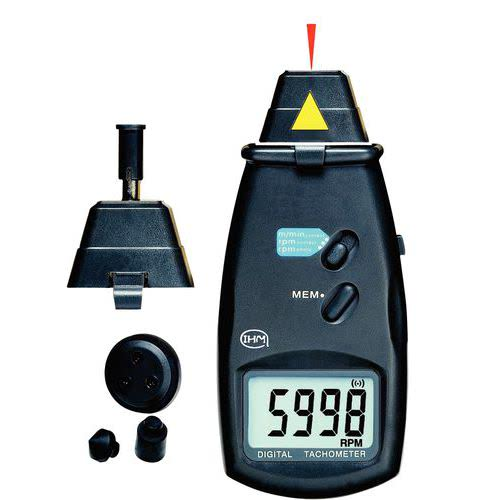
\includegraphics[width=50mm]{Tachymetre.png}
			\caption{Tachymètre tel que celui que nous avons utilisée\label{overflow}}
	\end{figure}
Ces nombres sont malheureusement trop faibles car nous souhaitions une vitesse de rotation de $27 \text{ } \SI{}{\radian}\cdot\SI{}{\per\second}$. Nous avons été contraints de garder cette vitesse pour garder un couple suffisant. En effet, les motoréducteurs ayant une assez grande puissance sont trop chers, ce qui nous a obligé à privilégier le couple au détriment de la vitesse.
	
	\subsubsection{Mesure du couple de sortie du motoréducteur avec un dynamomètre}
\indent \indent Nous avons attaché un fil relié à un dynamomètre sur le côté de notre roue de telle manière que le fil s’est enroulé autour de l’axe de rotation lorsque nous avons mis le moteur en fonctionnement. En tenant le dynamomètre et en tirant de plus en plus fort dessus nous avons mesuré la force maximale délivrée par le motoréducteur sur l’arbre des roues, c’est-à-dire la force appliquée par le fil en opposition à la force du moteur telle que le mouvement est nul, qu’il  n’y a plus de rotation.
	\begin{figure}[ht!]
		\centering
			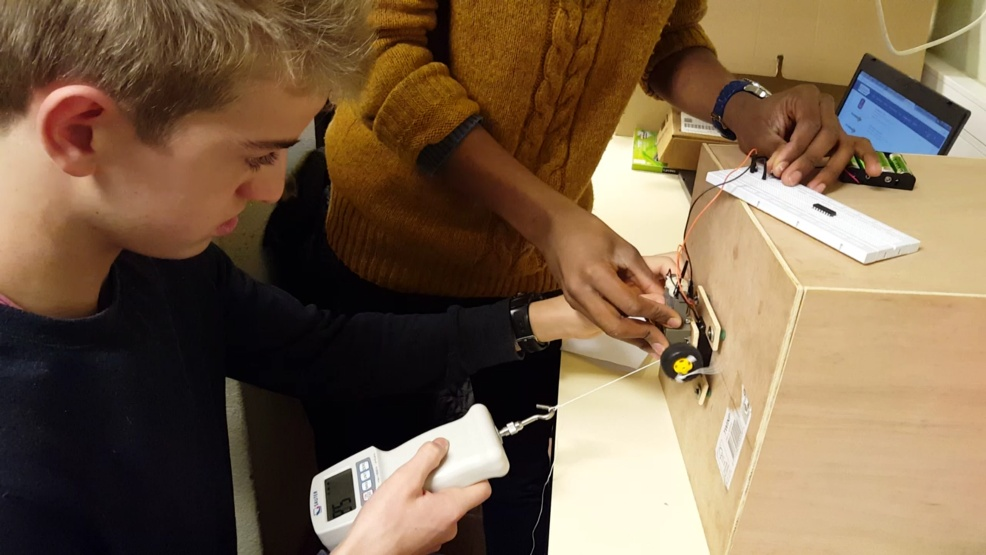
\includegraphics[width=100mm]{Mesure_couple.jpg}
			\caption{Mesure du couple du moteur avec un dynamomètre\label{overflow}}
	\end{figure}
	Nous avons mesuré une force de 35 Newtons, ce qui donne si on la multiplie par le rayon de la roue (sur laquelle nous avons fixé le fil) un couple $C = 35 \times 0,018 = 0,63 \text{ } \SI{}{\newton}\cdot\SI{}{\meter}$.
Ce couple est donc largement suffisant pour notre robot. (Il nous fallait $0,25  \text{ } \SI{}{\newton}\cdot\SI{}{\meter}$). 
Ainsi le motoréducteur pourra faire avancer notre robot lorsque sa masse est inférieure ou égale à $\SI{10}{\kilogram}$.
	
	\subsection{Électronique}
	
	Nous avons fait exactement la même chose que dans la partie simulée en branchant les câblages d’une manière plus ou moins définitive. En revanche, dans cette partie électronique nous avons rencontré certains problèmes.
	
	\subsubsection{Écran LCD}
	
	En effet, l’écran LCD destiné à la communication entre le robot et l’utilisateur nous a posé quelques soucis. Après une certaine maladresse, une chute de l’écran a engendré une cassure interne qui le rendait inutilisable. Nous fûmes donc contraints d’en racheter un autre qui, cette fois-là, fonctionna parfaitement.
	
	\subsubsection{Boutons poussoirs}
	
	Le câblage "pull down" des boutons poussoirs dans le système souhaité était erroné (nous n’avions en fait pas réalisé un câblage "pull down". Nous avons découvert notre erreur lors du montage du système réel car lorsque l’on appuyait sur un bouton le programme affichait que nous avions appuyé 2 ou 3 fois dessus. Nous avons donc modifié le câblage et rendu le bon fonctionnement des boutons.
	
	\subsubsection{Moteur à courant continu}
	
	Pour le moteur à courant continu (CC), nous avons rencontré d’autres sources de problèmes. Nous avions décidé dans un premier temps de prendre un système à deux moteurs CC indépendants pour un maximum de couple et pour qu’il convienne à nos attentes du cahier des charges. Une erreur de montage nous a alors contraint à acheter un nouveau modèle. De plus, ce qui était annoncé sur le site en termes d’informations liées aux capacités de ce moteur étaient fausses. C’est lors du test fait sur le système réel que nous nous sommes rendu compte du fait que les moteurs choisis ne suffisaient absolument pas à faire avancer la masse souhaitée. Nous avons donc choisi un moteur dont la fiche d’information semblait cette fois-ci correcte. De surcroît, le nouveau moteur permettait différentes configurations ce qui nous a permis de respecter un maximum le cahier des charges.
	
	\subsubsection{Moteur pas à pas}
	
	Étant donné que le driver et le moteur pas à pas constituaient des modèles particuliers nécessitant une programmation particulière, nous avons à plusieurs reprises pensé que ces derniers ne fonctionnaient pas. Après avoir réglé ces problèmes de programmation, cela fonctionnait parfaitement et il n’y avait donc en fait aucun problème concernant le moteur pas à pas et son driver.
	
	\subsubsection{Servomoteurs}
	
	Pour les servomoteurs, les problèmes furent nombreux : nous avions au départ récupéré deux servomoteurs d’une voiture radiocommandée d’un des membres du groupe. Cependant, après un certain temps, l’un d’entre eux s’est mis à dysfonctionner, probablement à cause d’une intensité trop importante lors d’un test sur le système réel. Cela nous a alors conduit à le remplacer par un neuf. Quelque temps après, le second servomoteur a lui aussi commencé à ne fonctionner correctement, cette fois-ci pour une raison inconnue. Nous avons donc dû acheter à nouveau un modèle neuf, identique à celui dont il était question précédemment.
	\newpage
	\section{Programmation}
	
	\indent\indent En ce qui concerne la programmation, le projet utilise plusieurs langages \nolinebreak: Python, pour le code du robot ainsi que pour le programme version ordinateur, Java, pour l'application Android, ainsi que HTML, CSS, Javascript et PHP pour le site internet, avec également des requêtes SQL pour accéder à la base de données de ce dernier.
	
	\subsection{Robot}
	
	\indent\indent Le robot utilise deux cartes éléctroniques pour fonctionner ; le code de ces dernières est donc distinct. La présentation de son code est donc divisée en deux parties : l'une pour le Raspberry Pi, programmé en Python, et l'autre pour l'Arduino, programmé en un dérivé du C. 
	
	\subsubsection{Raspberry Pi}
	
	\paragraph{Présentation}\mbox{}\\
	\subparagraph{Python}\mbox{}\\
\indent\indent Pour la programmation du Raspberry Pi, nous avons utilisé le langage de programmation interprété Python. Interprété signifie qu’il ne nécessite pas d’étape de compilation pour être exécuté. En effet, il est traduit en langage machine lors de son exécution par l’interpréteur CPython, contrairement à un langage compilé (comme le C ou le C++), qui doit lui être traduit en langage machine lors de son développement, mais ne nécessite pas de l'être à nouveau lors de son exécution.

\subparagraph{Programmation Orientée Objet}\mbox{}\\
\indent\indent Nous avons également décidé d’utiliser un paradigme (une technique) de programmation appelée Programmation Orientée Objet (POO). Cela conduit à la création, dans le code, de ce que l'on appelle des objets. Ces derniers sont des entités dans le programme qui possèdent plusieurs attributs :

- Des variables, pouvant être modifiées directement ou via une fonction interne à l'objet

- Des fonctions, ayant les mêmes capacités que les fonctions externes à l'objet et pouvant donc réaliser toutes sortes d'opérations, y compris modifier ou donner la valeur des variables de cet objet

Ces objets peuvent représenter n’importe quel objet ou entité du monde réel (ou imaginaire) ; ainsi, l’un des objets peut représenter un Arduino, un écran LCD ou un menu.
C’est ce que nous avons fait ici, comme vous pourrez le voir aux parties concernant les fichiers arduino.py, lcd.py ou menu.py.\\[0cm]
	
	Pour continuer sur le code du Raspberry Pi, voici un lien permettant d'accéder au code source du programme du Raspberry Pi, entièrement commenté, ce dernier étant trop long pour être inclus dans ce dossier :
	\begin{center}
	\url{https://github.com/thaspdev/PATRICK/tree/master/code/Raspberry\%20Pi}
	\end{center}
	
	Ce dernier est composé de 8 fichiers : 
	
	- patrick.py, fichier principal du programme, permettant notamment la communication entre les différents threads;
	
	- arduino.py, lcd.py et menu.py, contenant des objets;
	
	- communication\_arduino.py, permettant de communiquer avec le programme de l'arduino;
	
	- détection\_visage.py, code permettant de repérer les visages des utilisateurs du robot;
	
	- gestionnaire\_menu.py, permettant de contrôler le menu affiché sur l'écran LCD;
	
	- communication\_bluetooth.py, permettant de communiquer des messages à l'application Android ainsi que d'en recevoir en sa provenance.
	
	Nous présenterons tout de même ici quelques informations importantes concernant le code de certains fichiers.	
	
	\paragraph{patrick.py}\mbox{}\\
	
	\subparagraph{Division du programme en threads}\mbox{}\\
	
	Afin de pouvoir exécuter plusieurs actions en parallèle, nous avons dû diviser le programme en threads (aussi appelés tâches en français). Chaque thread est un ensemble d'instructions pouvant être exécutées en parallèle, dans la limite des capacités de l’ordinateur et du GIL (Global Interpreter Lock) de CPython, verrou informatique, limitant donc l’accès aux ressources de l’ordinateur.
	
	\subparagraph{Queues permettant la communication entre les threads}\mbox{}\\
	
	Pour assurer la communication entre les différents threads du programme, il a fallu utiliser ce que l’on appelle des queues (terme anglais), ou files en français, qui sont des structures de données (une structure de données correspond à une façon de ranger et d’accéder à des données) fondées sur le principe du Premier Entré Premier Sorti (PEPS), ou First In First Out (FIFO) en anglais. Cela signifie que la première donnée entrée dans cette queue sera la première à en sortir. Dans ce cas-là, nous avons dû utiliser deux queues par thread. En effet, le premier des deux sert à effectuer des communications (en mettant des messages dans la queue) entre patrick.py et le thread en question, et le second fait l’inverse, comme le montre le schéma suivant :
	
	\begin{figure}[ht!]
		\centering
			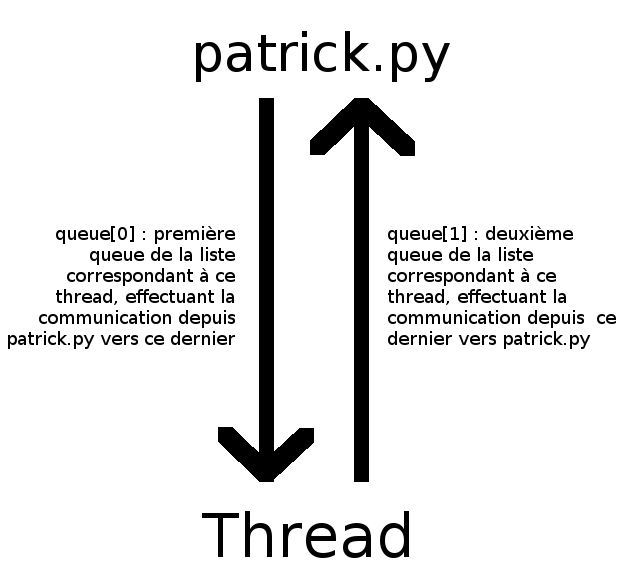
\includegraphics[width=100mm]{schema_communication_queues.png}
			\caption{Schéma de la communication via une queue entre patrick.py et un thread\label{overflow}}
	\end{figure}
	
	\paragraph{détection\_visage.py}\mbox{}\\
	
	Pour bien déterminer l'angle auquel le robot aurait dû tourner, il aurait fallu connaître certaines informations à propos de la caméra, informations dont nous ne disposions pas. Nous n'avons donc pas pû réaliser une estimation totalement effective de ce dernier. Pour réaliser cette détection de visages, nous avons utilisé OpenCV, un module notamment disponible sous Python permettant, entre autres, de reconnaître des objets dans une image grâce au deep learning.
	
	\paragraph{communication\_bluetooth.py}\mbox{}\\
	
	Nous avons utilisé pour la programmation de ce code le module bluez (aussi appelé pybluez dans sa version Python).
	
	
	\subsubsection{Arduino}
	
\indent\indent Le principe du code de l'Arduino, dans ce TPE, est d'effectuer une boucle infinie et d'analyser le contenu des données qu'il reçoit en série, comme vous pourrez le voir à l'adresse :
	
	\begin{center}
		\url{https://github.com/thaspdev/PATRICK/code/Arduino}
	\end{center}

\subsection{Application Android}

\indent\indent L'application Android permet de répondre à la fonction technique 7 du robot, puisqu'elle permet de contrôler ce dernier depuis un smartphone.

N'est détaillé en ligne que le code de l'application Android duquel un lien avec le projet peut être dégagé. En effet, ce code est très long et concerne majoritairement le design de l'application ou la réponse à une action de l'utilisateur (par exemple, l'appui sur un bouton (de l'interface de l'application)), ce qui ne présente que peu d'intérêt pour ce TPE. L'ensemble du code de cette application est disponible à l'adresse suivante \nolinebreak:

\begin{center}
	\url{https://github.com/thaspdev/PATRICK_Android}
\end{center}

\subsection{Site internet}

\indent\indent Nous avons réalisé un site internet pour ce TPE, notamment afin de faciliter la communication entre les membres du groupe pour ce qui est du dossier. Cependant, comme pour l'application Android, son code est très long et son intérêt par rapport au projet est, de plus, moindre. Son fonctionnement ne sera donc pas détaillé en ligne, mais son code est consultable dans son intégralité à l'adresse suivante :
	
	\begin{center}
	\url{https://github.com/thaspdev/PATRICK_Web}
	\end{center}
	\newpage
	\section{Idées d'amélioration}
	
	\indent\indent Nous n'avons malheureusement pas pu intégrer toutes les idées que nous avions au robot, que ce soit par manque de moyens ou pour d'autres raisons. Ainsi, nous avons par exemple réfléchi à un système d'évitement d'obstacles et de localisation (du robot en lui-même, et non pas de la personne) par ultrasons, ou un système de soulèvement du plateau supportant les objets actionné par une pédale. Nous ne les détaillons pas ici car ils ne font pas partie intégrante du projet, et, de plus, ils méritent d'être perfectionnés. Ces idées seront cependant disponibles à l'adresse suivante :
	
\begin{center}
	\url{https://github.com/thaspdev/PATRICK/ameliorations/}
\end{center}
	\newpage
	\section{Conclusion}
	
	\indent\indent En conclusion de ce projet, nous pourrions dire que nous l’avons trouvé enrichissant par bien des aspects. En effet, nous avons grâce à lui pu d’une part découvrir les bases de l’électronique, en nous formant sur un Arduino et en l’utilisant pour contrôler divers appareils électroniques, tels que des servomoteurs, un moteur pas à pas, un afficheur LCD ou encore un moteur à courant continu. Nous avions par ailleurs déjà étudié cet appareil en cours et nous pouvons dire que ce TPE nous a permis d’appliquer les connaissances acquises en cours, par exemple en ce qui concerne son couple et sa vitesse de rotation, ainsi que, parfois, de les approfondir, par exemple avec le calcul du couple du moteur en fonction notamment de la résistance au roulement des roues. Il nous a également permis de nous perfectionner dans la partie manuelle du projet, en partie composée de sa construction. De plus, nous avons également pu grâce à lui nous familiariser avec des outils usuels dans le milieu des Sciences de l’Ingénieur, tels que le tachymètre et le dynamomètre. De surcroît, nous avons ainsi pu avoir une meilleure perception de ce qu’est un système réel, ainsi que de toutes les étapes menant de la définition du cahier des charges jusqu’à la production du robot, en passant par le bureau d’études. Nous regrettons cependant que la modification du cahier des charges en ce qui concerne les ultrasons ait abaissé la part de Sciences Physiques présente dans ce TPE. Quoi qu'il en soit, bien que le TPE ne soit, au moment au nous écrivons ce rapport, pas encore totalement abouti, il a été une expérience très intéressante que nous serions prêts à refaire si l'occasion nous en était donnée.
	\newpage
	\section{Annexes}
	
	\subsection{Photographies}
	
\indent\indent Des photographies réalisées dans le cadre de ce TPE seront disponibles à cette adresse :
	
	\begin{center}
	\url{https://github.com/thaspdev/PATRICK/tree/master/photos}
	\end{center}
	
	\subsection{Vidéos de test du robot}
	
\indent\indent Nous posterons d'ici la soutenance orale de ce TPE des vidéos de test qui seront disponicles à l'adresse suivante :
	
	\begin{center}
	\url{https://github.com/thaspdev/PATRICK/tree/master/videos}
	\end{center}
	
	\subsection{Circuits électroniques}
	
\indent\indent Nous avons réalisé différents circuits électroniques sous Fritzing, un logiciel (libre) permettant nottament de modéliser ces mêmes circuits ; ainsi, nous vous les présentons les liens permettant d'y accéder ci-après (les fichiers FZZ sont des fichiers Fritzing et le PNG sont les exporations de ces derniers en images au format PNG) :
	
	- Schéma du branchement de l'écran LCD au Raspberry Pi : \url{https://github.com/thaspdev/PATRICK/tree/master/circuits/Raspi_lcd}
	
	- Schéma du branchement des boutons poussoirs au Raspberry Pi : \url{https://github.com/thaspdev/PATRICK/tree/master/circuits/Raspi_poussoir}
	
	- Schéma du câblage du moteur à courant continu à l'Arduino : \url{https://github.com/thaspdev/PATRICK/tree/master/circuits/Arduino_moteur}
	
	- Schéma du câblage du moteur pas à pas à l'Arduino : \url{https://github.com/thaspdev/PATRICK/tree/master/circuits/Arduino_stepper}
	
	- Schéma du câblage d'un des servomoteurs à l'Arduino : \url{https://github.com/thaspdev/PATRICK/tree/master/circuits/Arduino_servo}
\newpage
	
	\section{Bibliographie, références}
	
	\listoffigures
	
	\listoftables
	
\end{document}